\newpage

\section{Results and discussion}
\label{Sec:Results}

In this section, the results for the \pT-dependent non-linear flow modes $v_{4,22}$, $v_{5,32}$, $v_{6,33}$ and $v_{6,222}$ of identified particles are presented for various centrality intervals in Pb--Pb collisions at \sNN. We first present the centrality and \pT~dependence of $v_{n,mk}$ in Sec. \ref{SubSec:pTdependence}. The scaling properties of non-linear flow modes are also discussed in this section. Comparisons to two model calculations are shown in Sec. \ref{SubSec:hydro}. Finally, these results are compared with $v_{n}$ measurements in Sec. \ref{SubSec:comparewithvn}. Note that the same data are used in different representations to highlight the physics implications of the measurements in each section. 
%~for 0-5\% up to 50-60\% centrality intervals for \pion, \kaon, \proton, \Ks, \lambdas~and $\phi$-meson

\subsection{Centrality and \pT~dependence of non-linear flow modes}
\label{SubSec:pTdependence}

%Higher order flow coefficients are mainly generated by inhomogeneities in the initial density profile and the collision geometry. 
Figure \ref{v422_centralityDependence} presents the magnitude of the non-linear mode for the fourth order flow coefficient, $v_{4,22}(p_{\rm{T}})$, for \pion, \kaon,\Ks, \proton, \lambdas~and $\phi$-meson in a wide range of centrality intervals, i.e. 0-5\% up to 50-60\%. For $\phi$-meson, the results are reported from 10-20\% up to 40-50\% centrality interval, where $v_{4,22}$ can be measured accurately. The magnitude of this non-linear flow mode rises steeply with increasing centrality interval from 0-5\% to 40-50\% for all particle species. This increase is expected as $v_{4,22}$ measures the contribution of the second order eccentricity, $\varepsilon_{2}$, in $v_{4}$ which increases for peripheral collisions \cite{Alver:2010gr, Acharya:2017zfg}. For more peripheral collisions (i.e. 50-60\%) , the magnitude of $v_{4,22}$ is smaller than in the previous centrality intervals for all particle species. This effect that was observed also in $v_n$ measurements is probably due to the shorter lifetime of the produced system in more peripheral collisions, which prevents $v_{4,22}$ from developing further. 


\begin{figure}[!htb]
\begin{center}
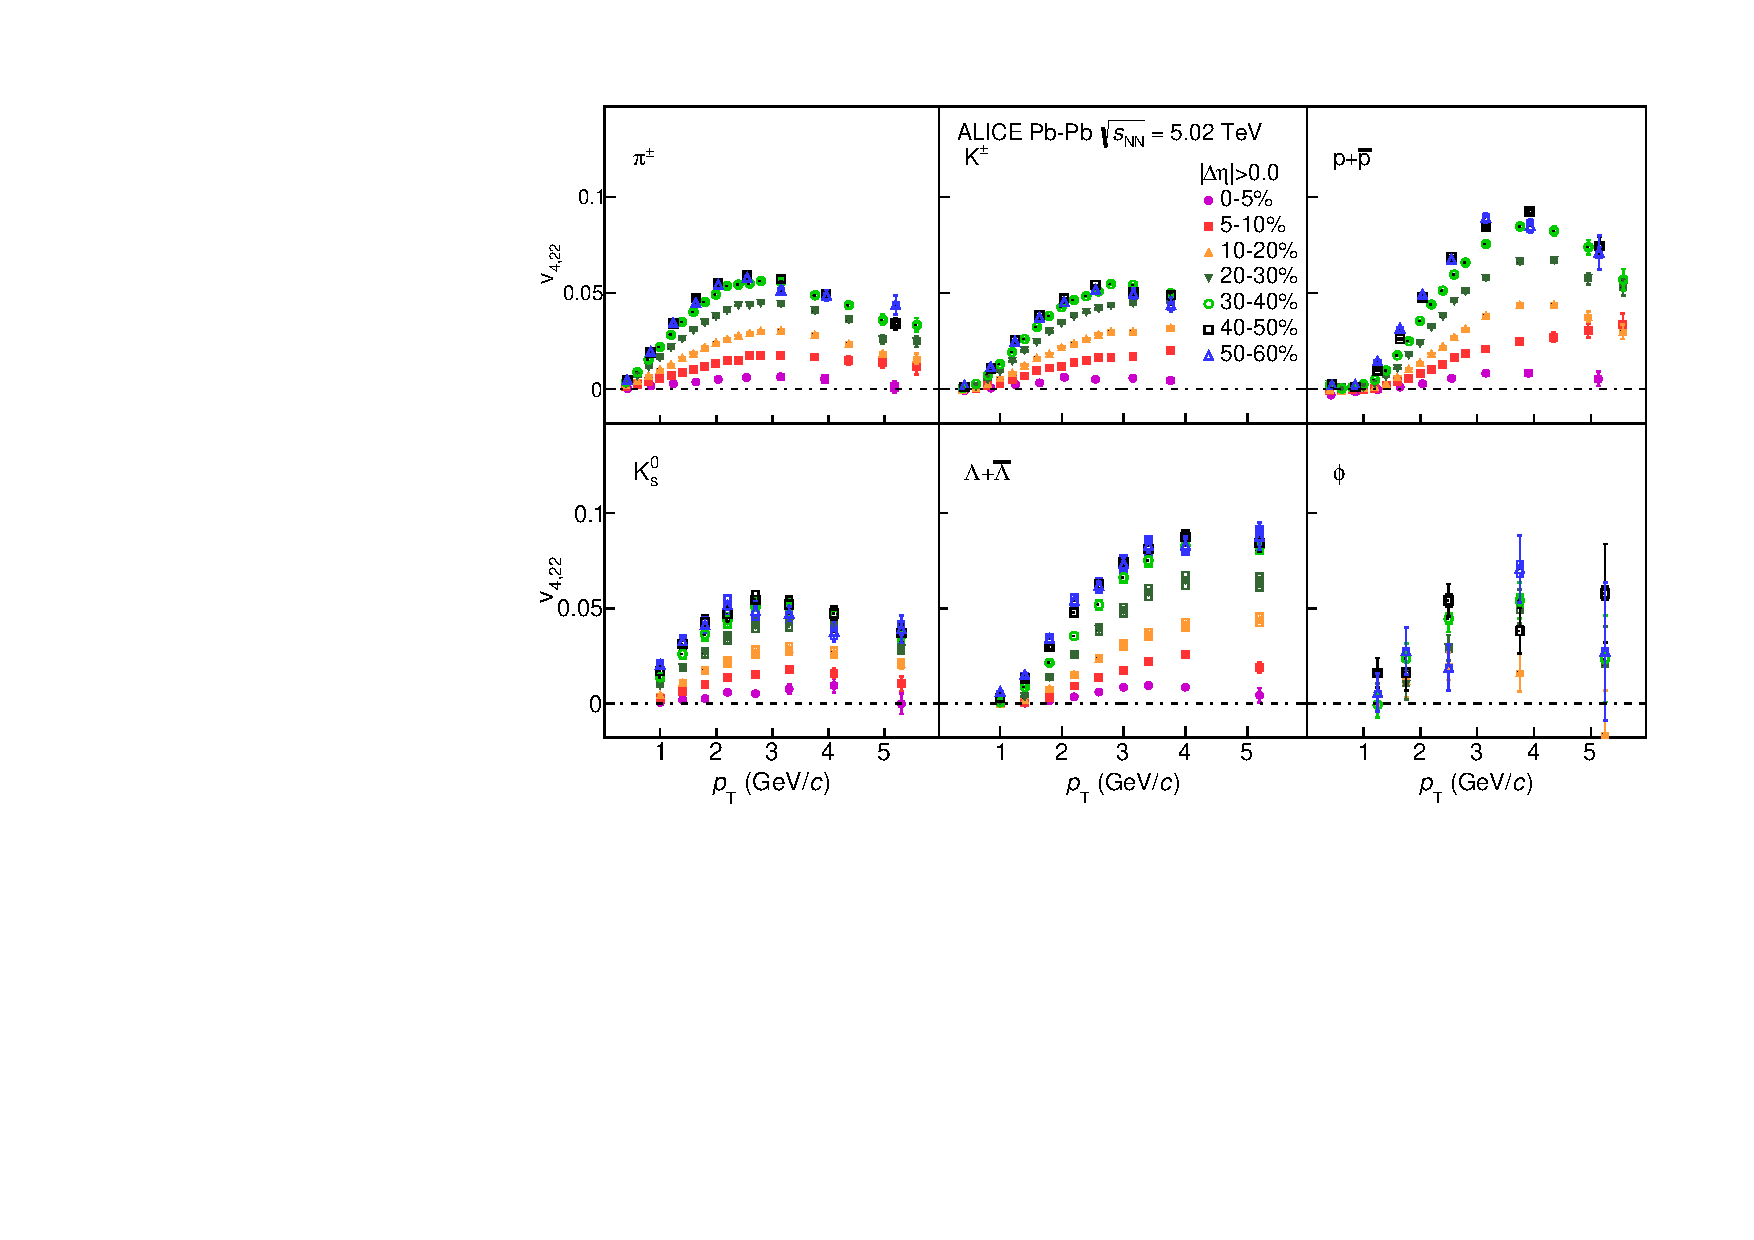
\includegraphics[scale=0.82]{figures/results/All_v422_gap00_CentDep_PID2.pdf}
\end{center}
\caption{The \pT-differential $v_{4,22}$ for different centrality intervals of Pb--Pb collisions at \sNN~ grouped by particle species. Statistical and systematic uncertainties are shown as bars and boxes, respectively.}
\label{v422_centralityDependence}
\end{figure}
 
Figure \ref{v523_centralityDependence} presents the non-linear mode for the fifth order flow coefficient, i.e. $v_{5,32}(p_{\rm{T}})$, of \pion, \kaon, \Ks, \proton, and \lambdas~for the same range of centrality intervals, i.e. 0-5\% up to 50-60\%. Statistical precision limits extending the measurements of non-linear flow modes of $\phi$-meson for $n>4$. The measurements show a significant increase in the magnitude of this non-linear flow mode with increasing centrality percentile. This is due to the fact that $v_{5,32}(p_{\rm{T}})$ has a contribution from both $\varepsilon_{2}$ and $\varepsilon_{3}$. It is shown in MC studies that both $\varepsilon_{2}$ and $\varepsilon_{3}$ increase for peripheral collisions \cite{Alver:2010gr}. Although, this increase is less pronounced for $\varepsilon_{3}$.

\begin{figure}[!htb]
\begin{center}
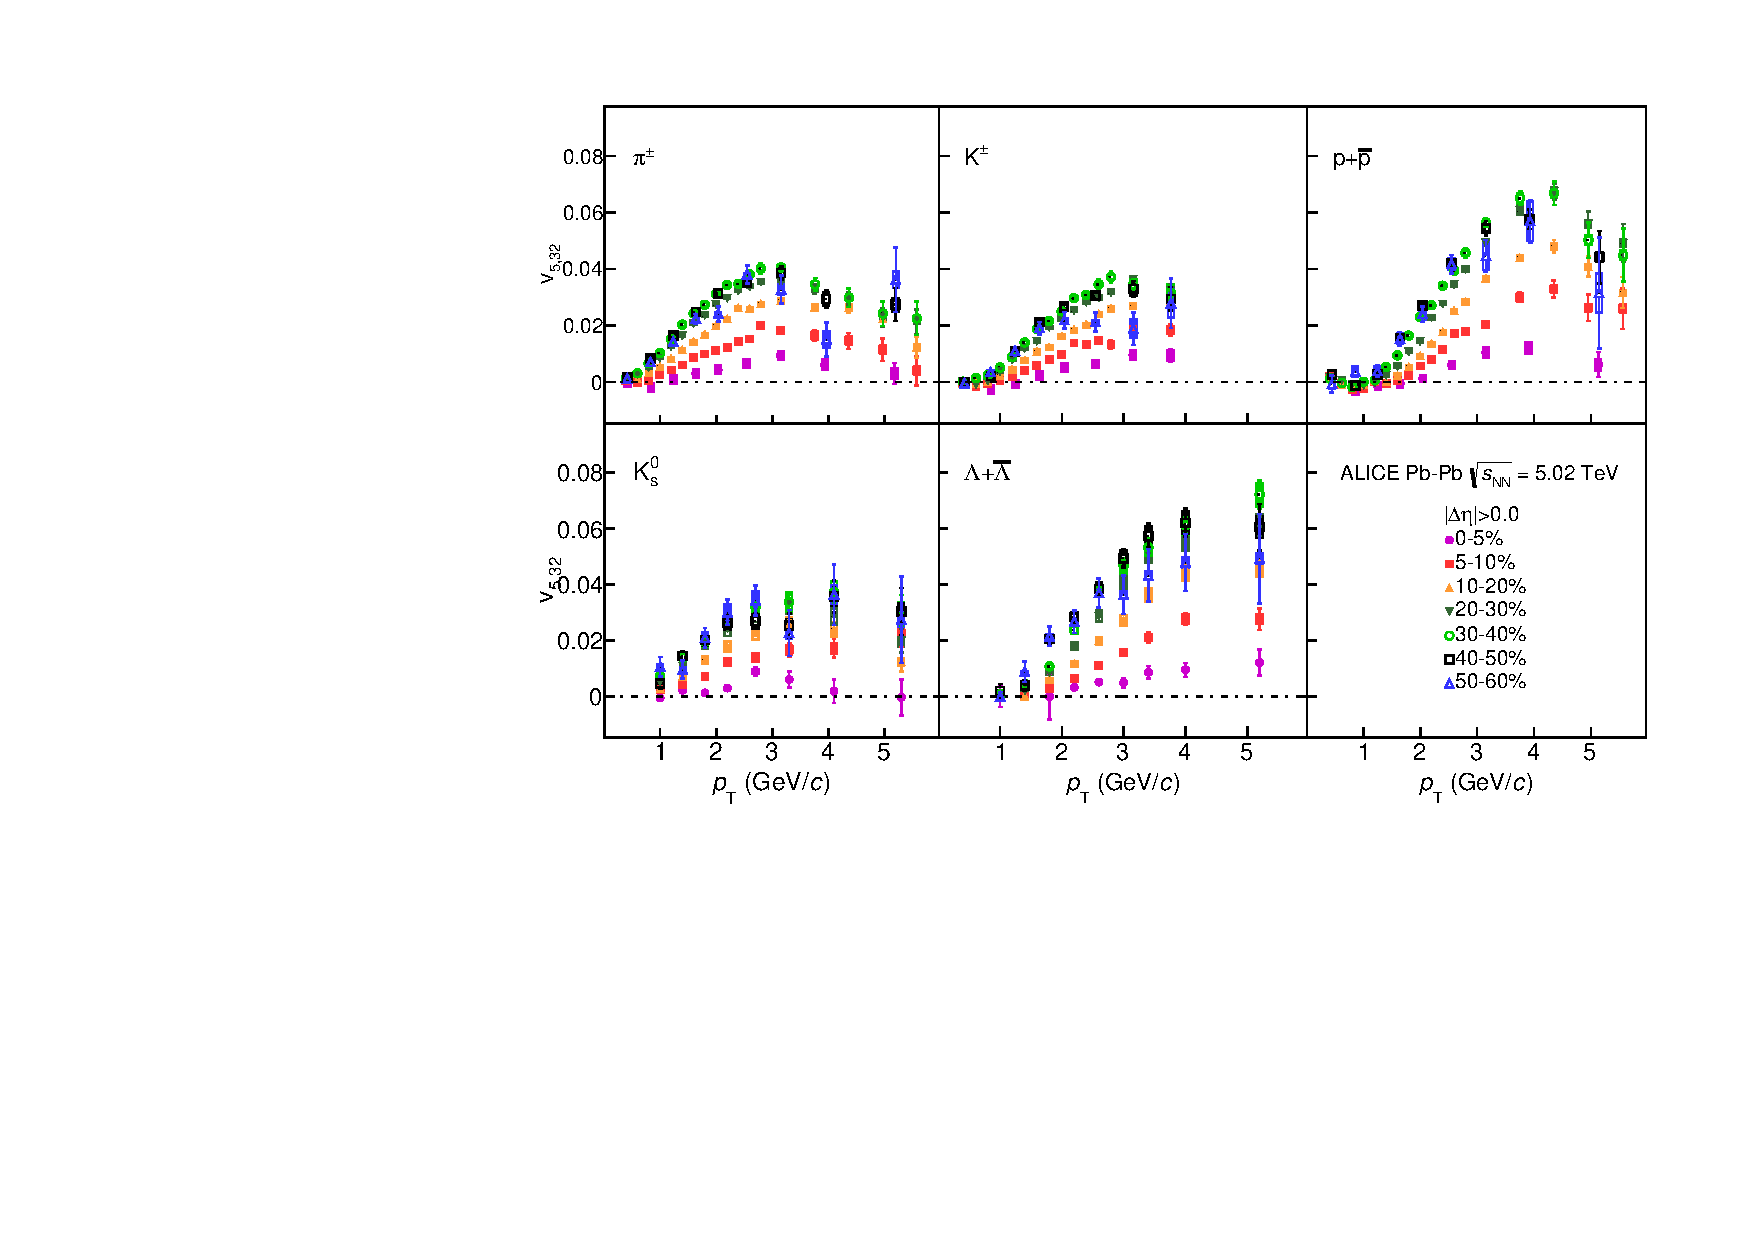
\includegraphics[scale=0.82]{figures/results/All_v523_gap00_CentDep_PID2.pdf}
\end{center}
\caption{The \pT-differential $v_{5,32}$ for different centrality intervals of Pb--Pb collisions at \sNN~ grouped by particle species.}
\label{v523_centralityDependence}
\end{figure}

Figures \ref{v633_centralityDependence} and \ref{v6222_centralityDependence} present the non-linear terms for the sixth order flow coefficient, i.e. $v_{6,33}(p_{\rm{T}})$ for \pion, \kaon, \Ks, \proton and \lambdas~and~at 0-5\% up to 40-50\% centrality intervals and $v_{6,222}(p_{\rm{T}})$ for \pion, \kaon, \proton~at 0-5\% up to 50-60\% centrality intervals. As expected, measurements of $v_{6,222}(p_{\rm{T}})$ show an increase in the magnitude of this non-linear flow mode with increasing centrality percentile, whereas, $v_{6,33}(p_{\rm{T}})$ presents little to no dependence on centrality \cite{Acharya:2017zfg}. 

\begin{figure}[!htb]
\begin{center}
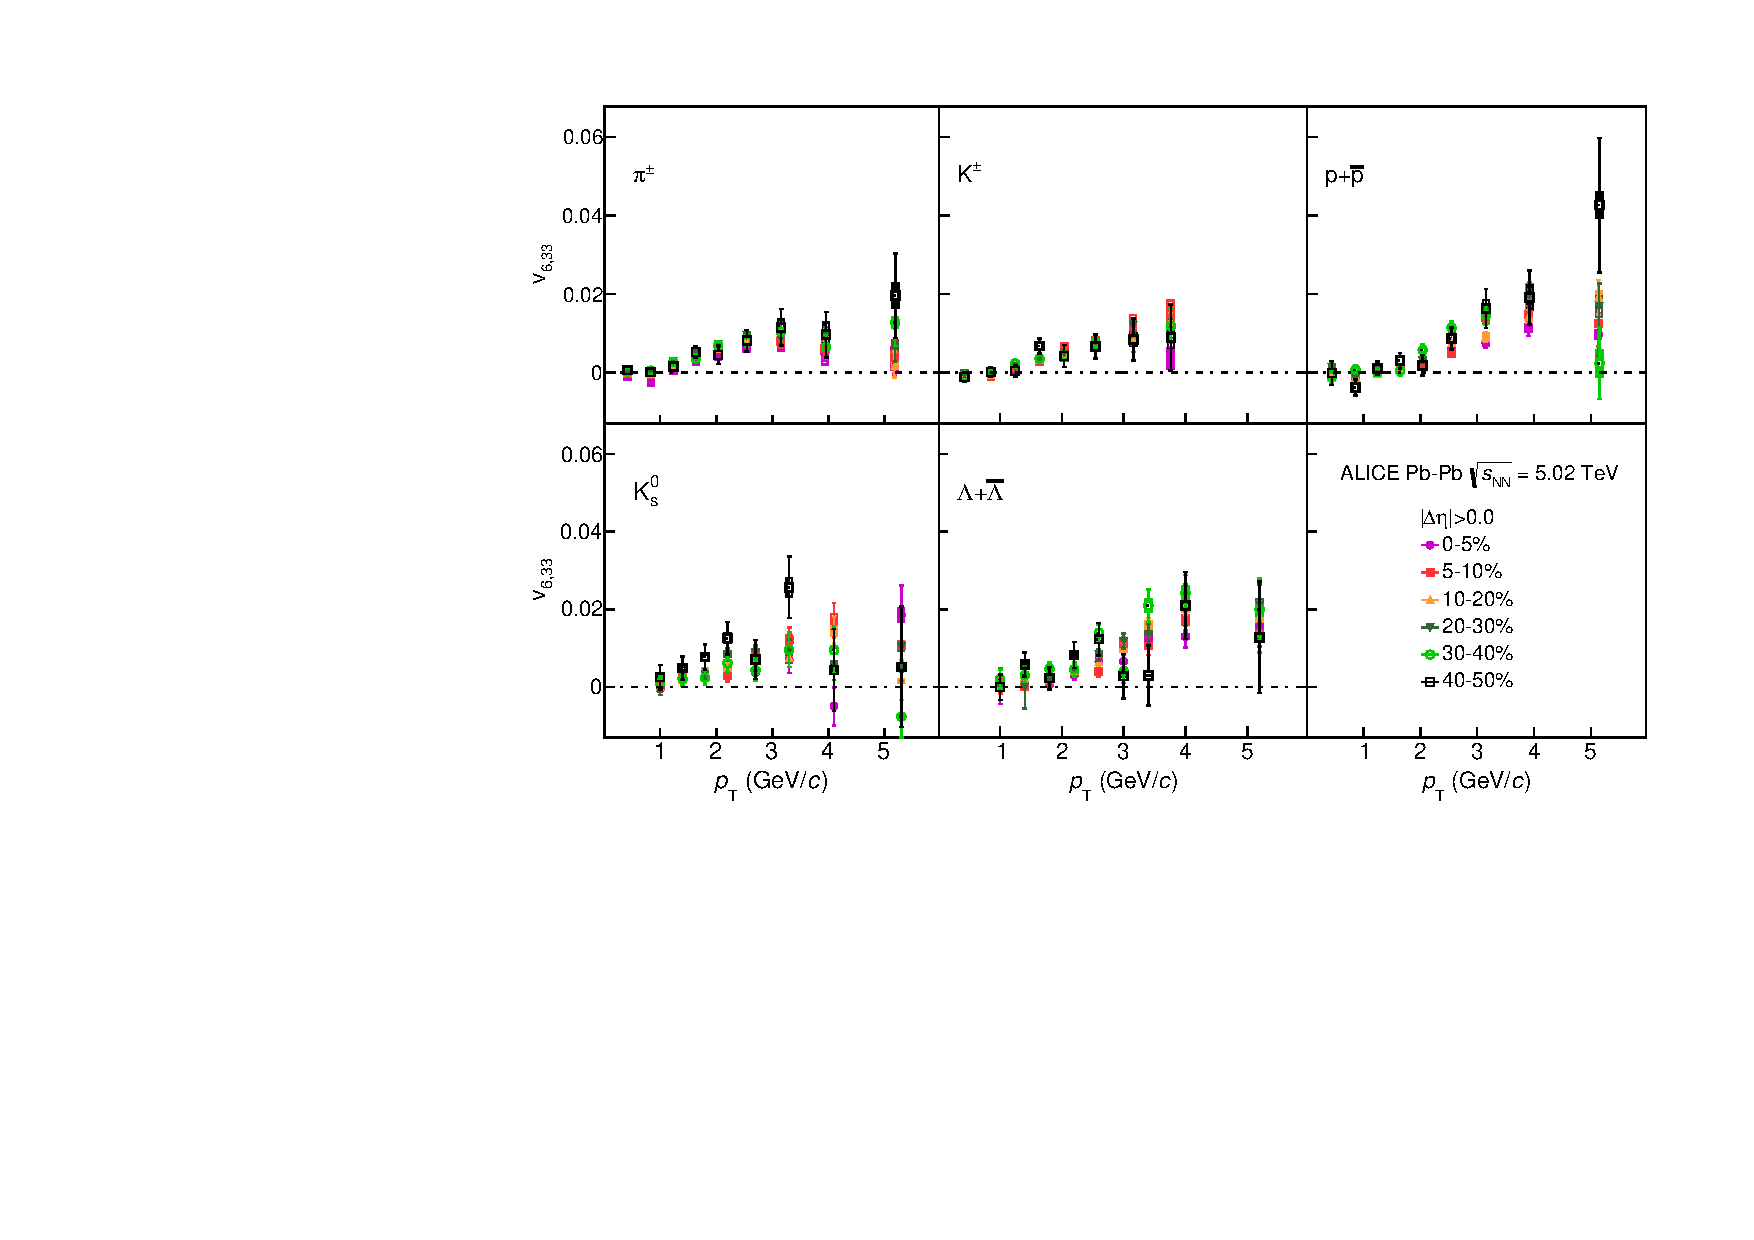
\includegraphics[scale=0.82]{figures/results/All_v633_gap00_CentDep_PID2.pdf}
\end{center}
\caption{The \pT-differential $v_{6,33}$ for different centrality intervals of Pb--Pb collisions at \sNN~ grouped by particle species.}
\label{v633_centralityDependence}
\end{figure}

\begin{figure}[!htb]
\begin{center}
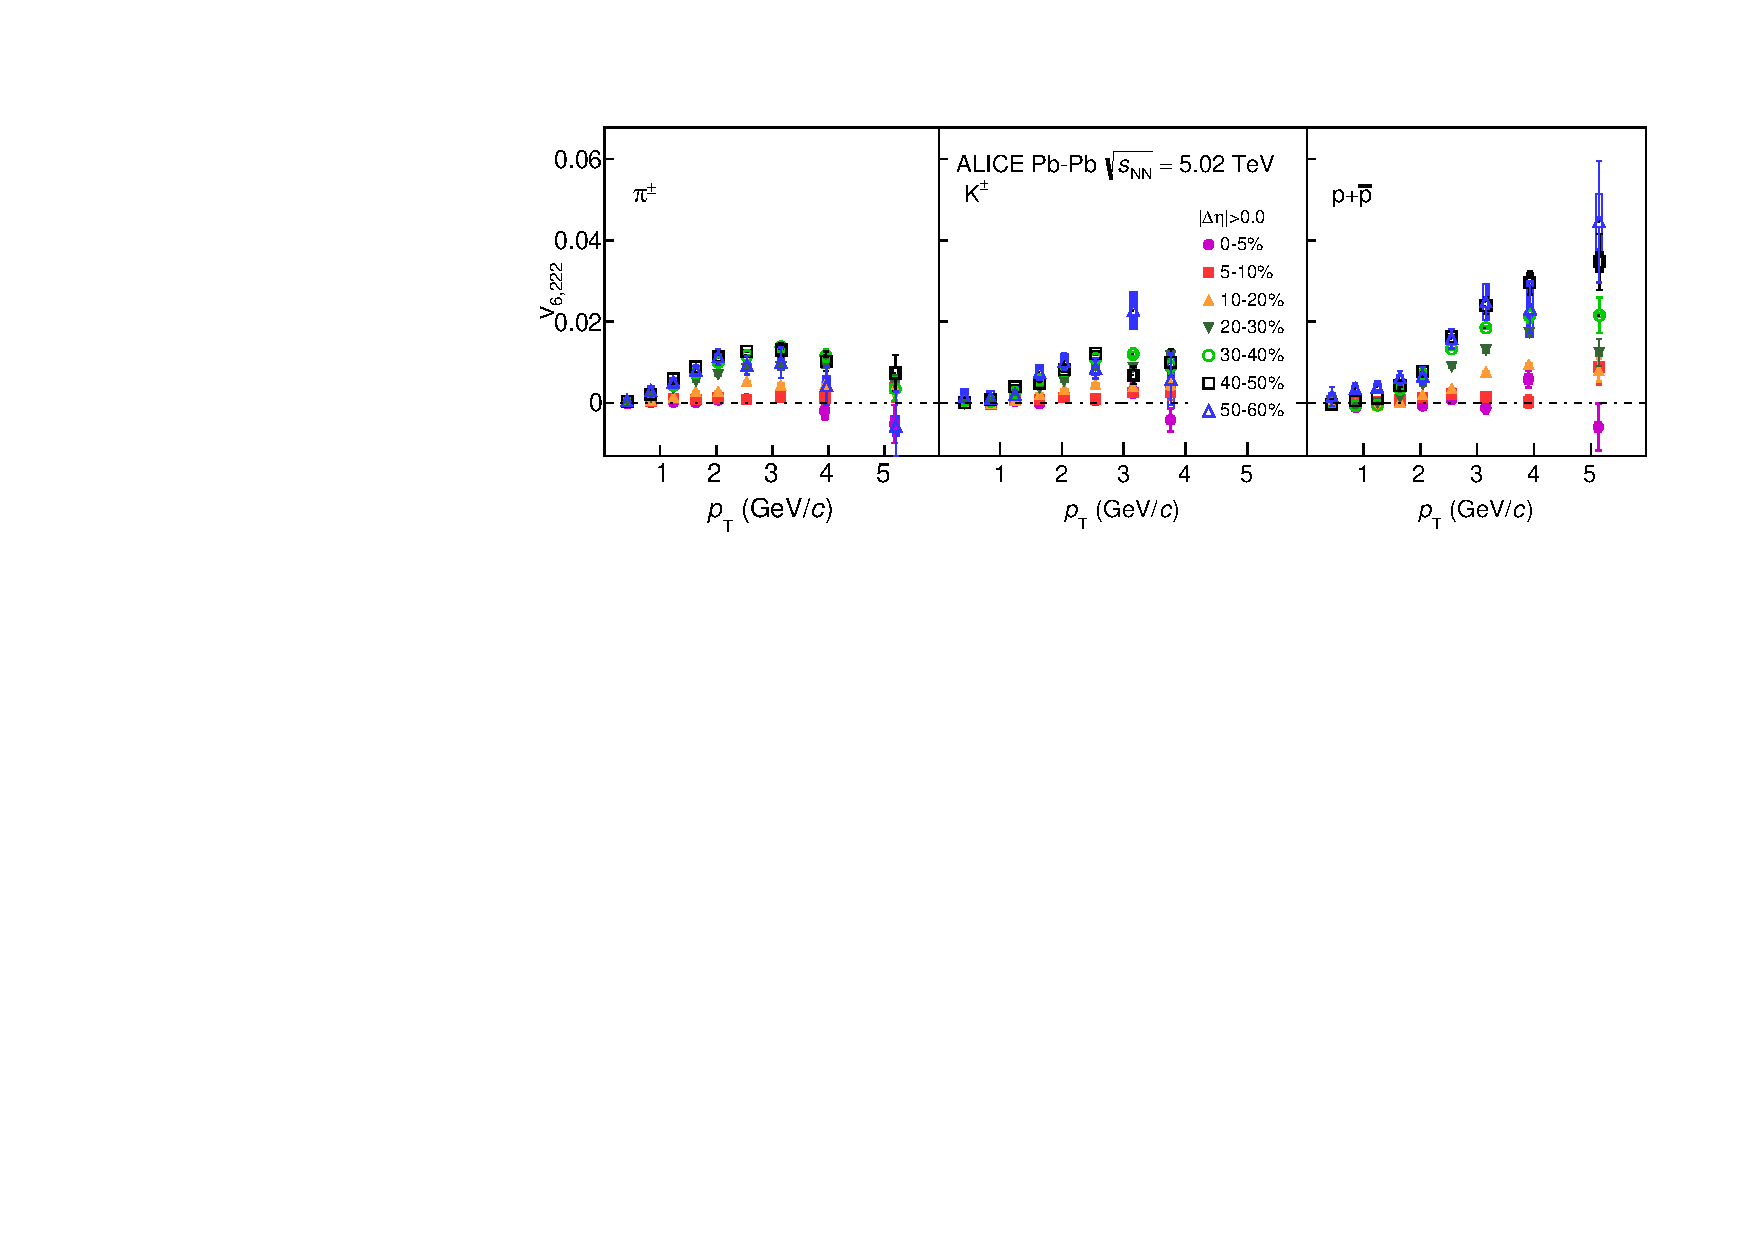
\includegraphics[scale=0.82]{figures/results/All_v6222_gap00_CentDep_PID2.pdf}
\end{center}
\caption{The \pT-differential $v_{6,222}$ for different centrality intervals of Pb--Pb collisions at \sNN~ grouped by particle species.}
\label{v6222_centralityDependence}
\end{figure}

\newpage
%\subsection{Mass ordering}
%\label{MassOrdering}

In Fig. \ref{v422_particleDependence} the same data points are grouped by centrality interval to highlight how $v_{4,22}$ develops for a given centrality for various particle species as a function of \pT.
%Figures \ref{v422_particleDependence} presents the \pT-differential $v_{4,22}$ for \pion, \kaon, \proton, \Ks, \lambdas~and $\phi$-meson starting from most central collisions (0-5\%) up to the 50-60\% centrality interval. 
A clear mass ordering can be seen in the low \pT~region (i.e. \pT $< 2.5$ \GeV) at all collision centralities. This mass ordering arises from the interplay between the anisotropic flow and radial flow. Radial flow creates a depletion in the particle spectra at lower \pT~values which leads to lower $v_{4,22}$ for heavier particles \cite{Voloshin:1996nv, Huovinen:2001cy, Shen:2011eg}.

\begin{figure}[!htb]
\begin{center}
%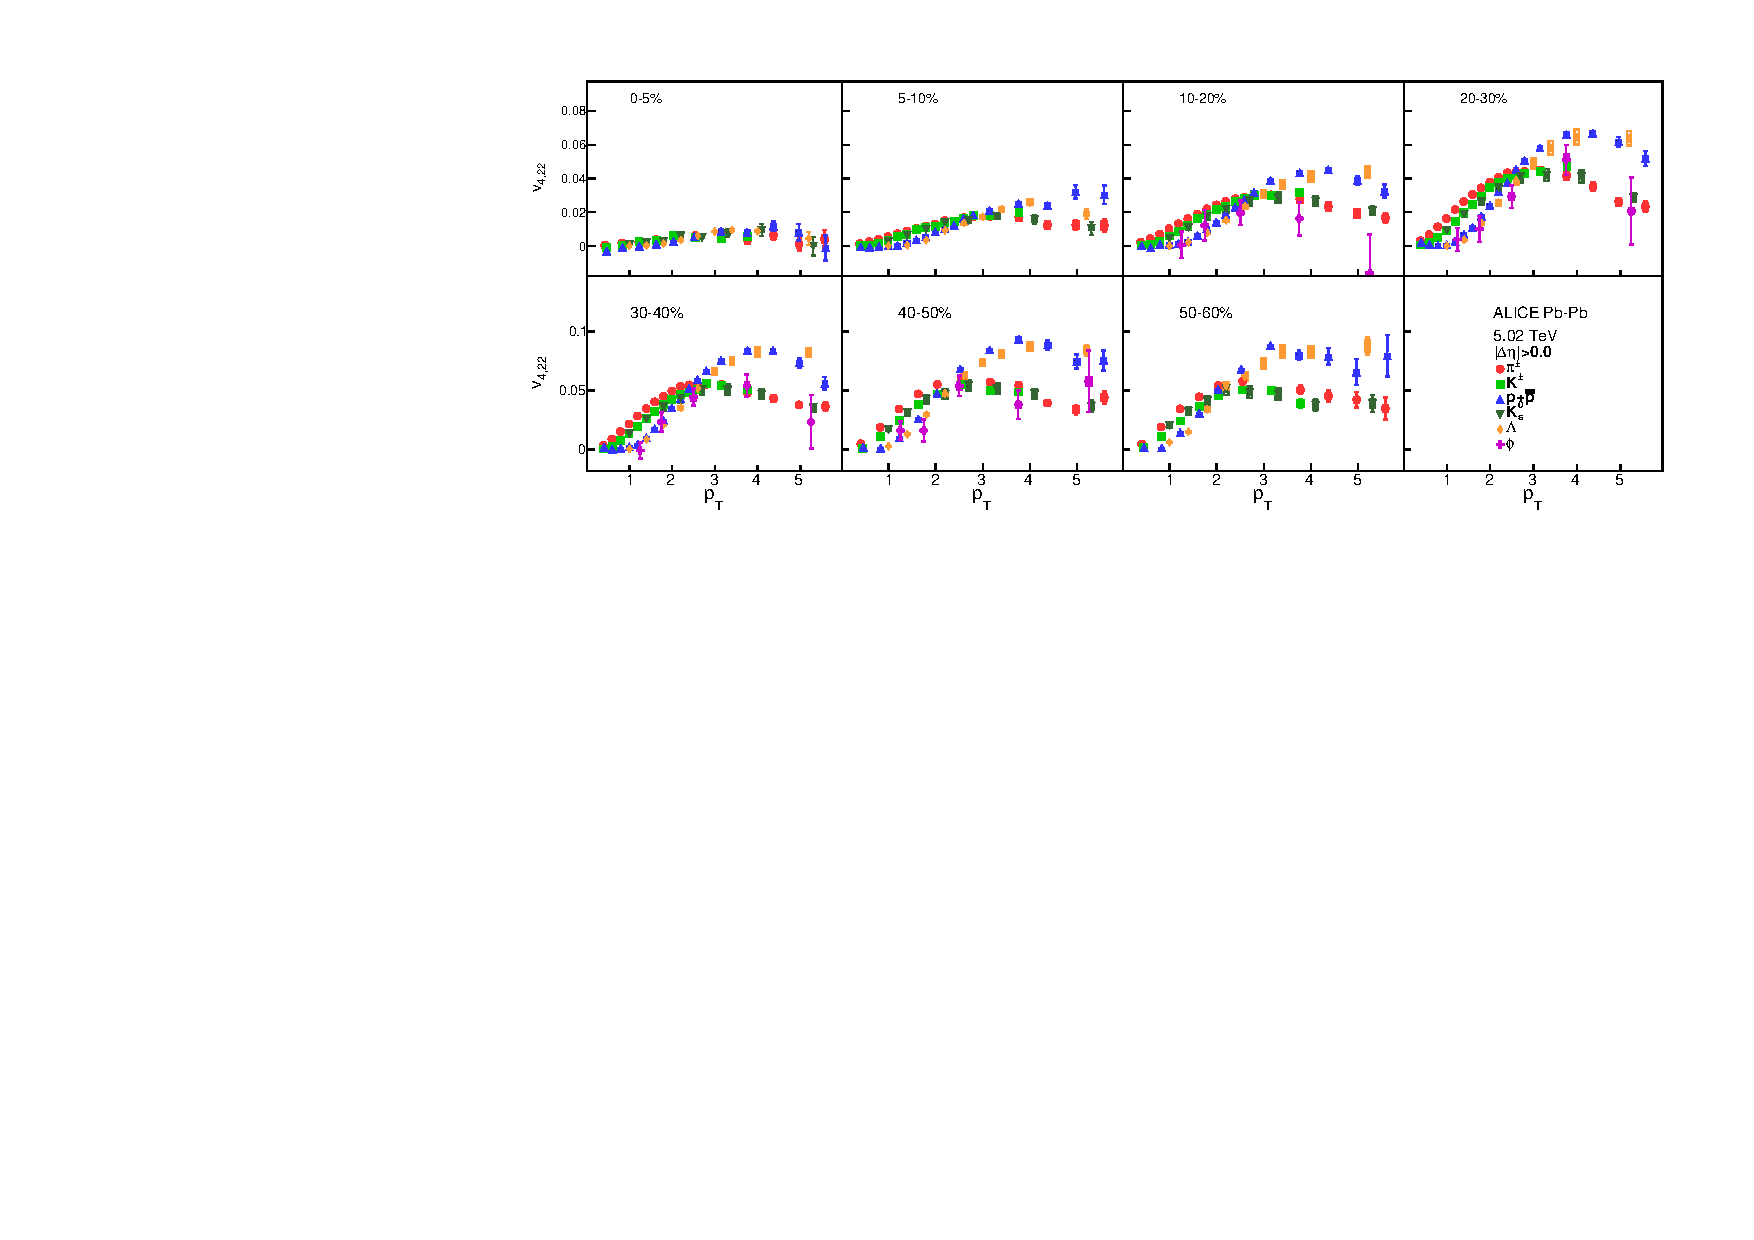
\includegraphics[scale=0.82]{figures/results/All_v422_gap00.pdf}
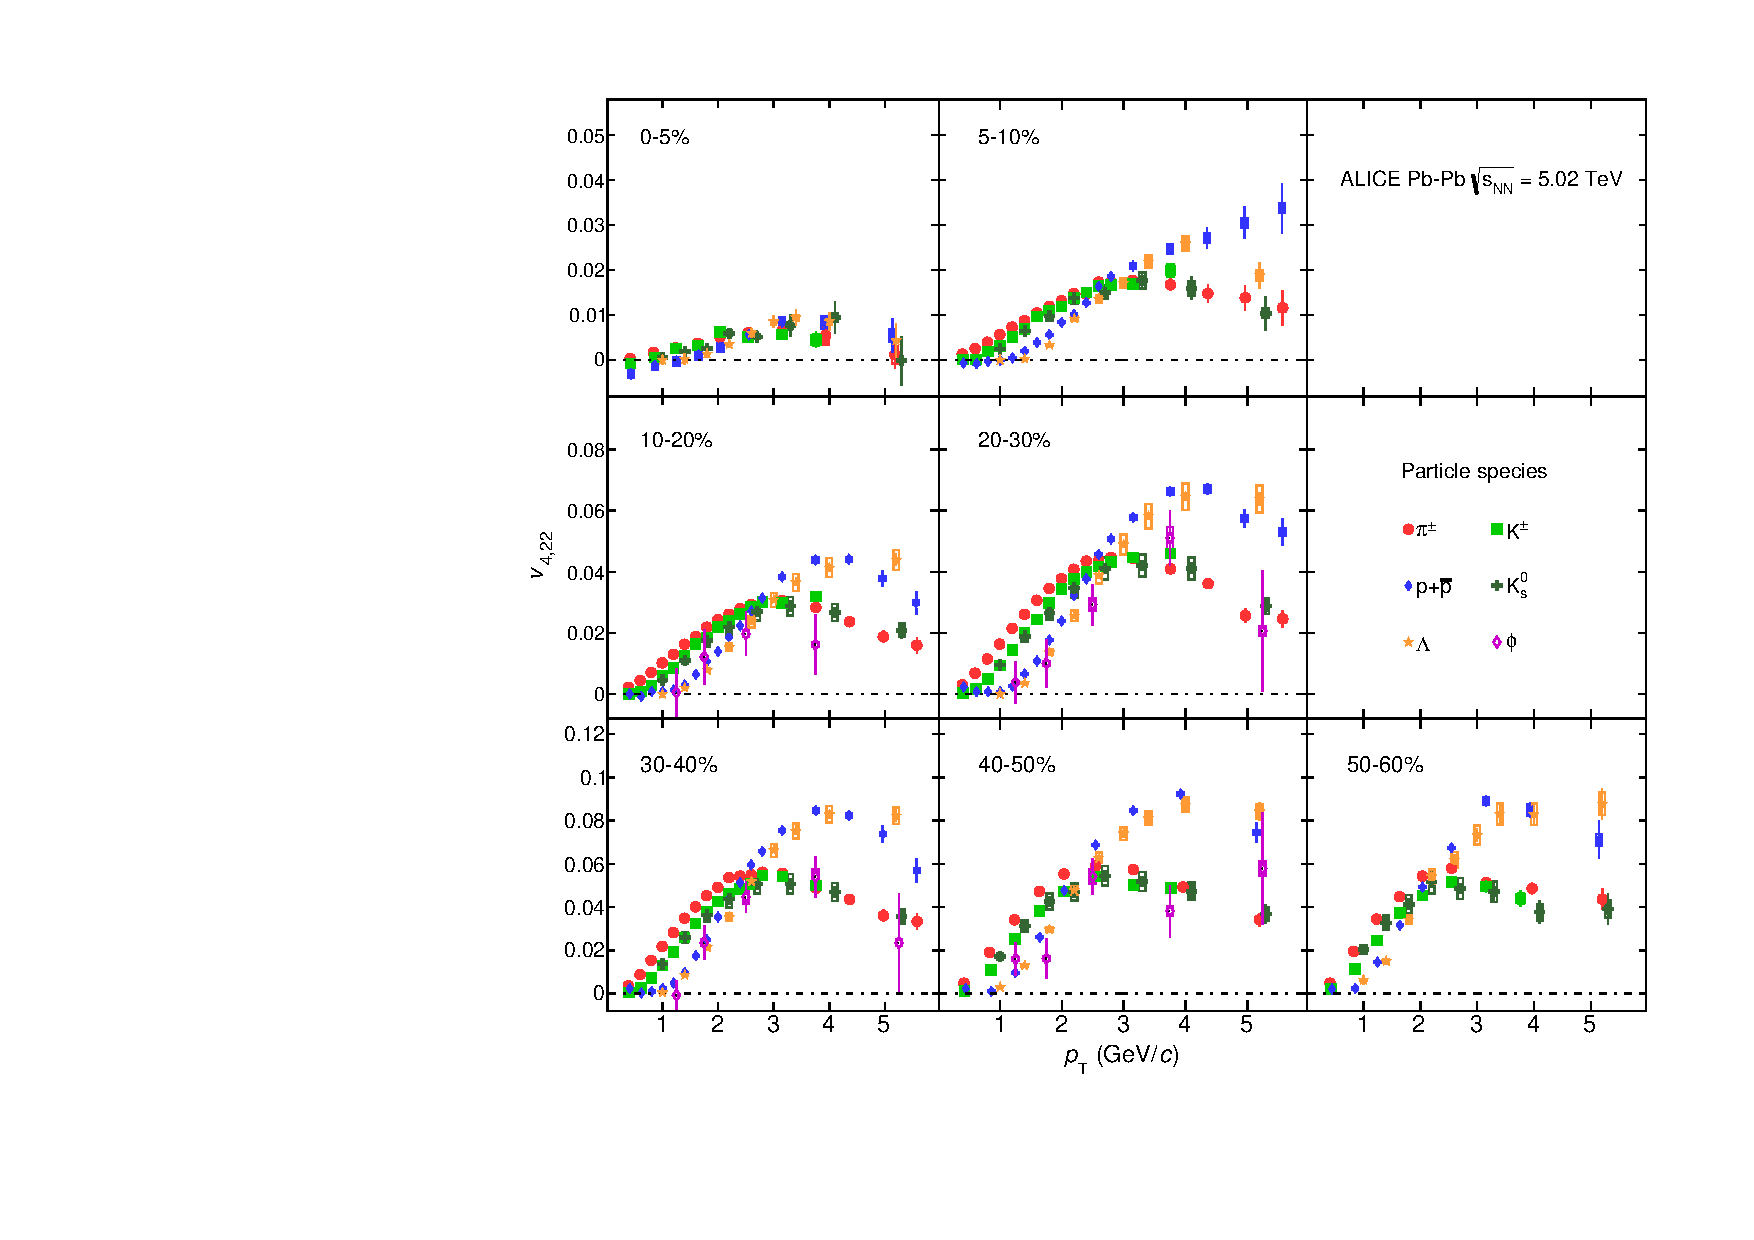
\includegraphics[scale=0.82]{figures/results/All_v422_gap00_PID2_3by3.pdf}
\end{center}
\caption{The \pT-differential $v_{4,22}$ for different particle species grouped into different centrality intervals of Pb--Pb collisions \sNN}
\label{v422_particleDependence}
\end{figure}

Similarly, Figs. \ref{v523_particleDependence}, \ref{v633_particleDependence} and \ref{v6222_particleDependence} show the \pT-differential $v_{5,32}$, $v_{6,33}$ and $v_{6,222}$ respectively, of different particle species for each centrality interval. A clear mass ordering is seen in the low \pT~region, (i.e. \pT $< 2.5$ \GeV), for $v_{5,32}(p_{\rm{T}})$, $v_{6,33}(p_{\rm{T}})$ and $v_{6,222}(p_{\rm{T}})$, which similarly arises from the interplay between the non-linear response of the system and radial flow. 

\begin{figure}[!htb]
\begin{center}
%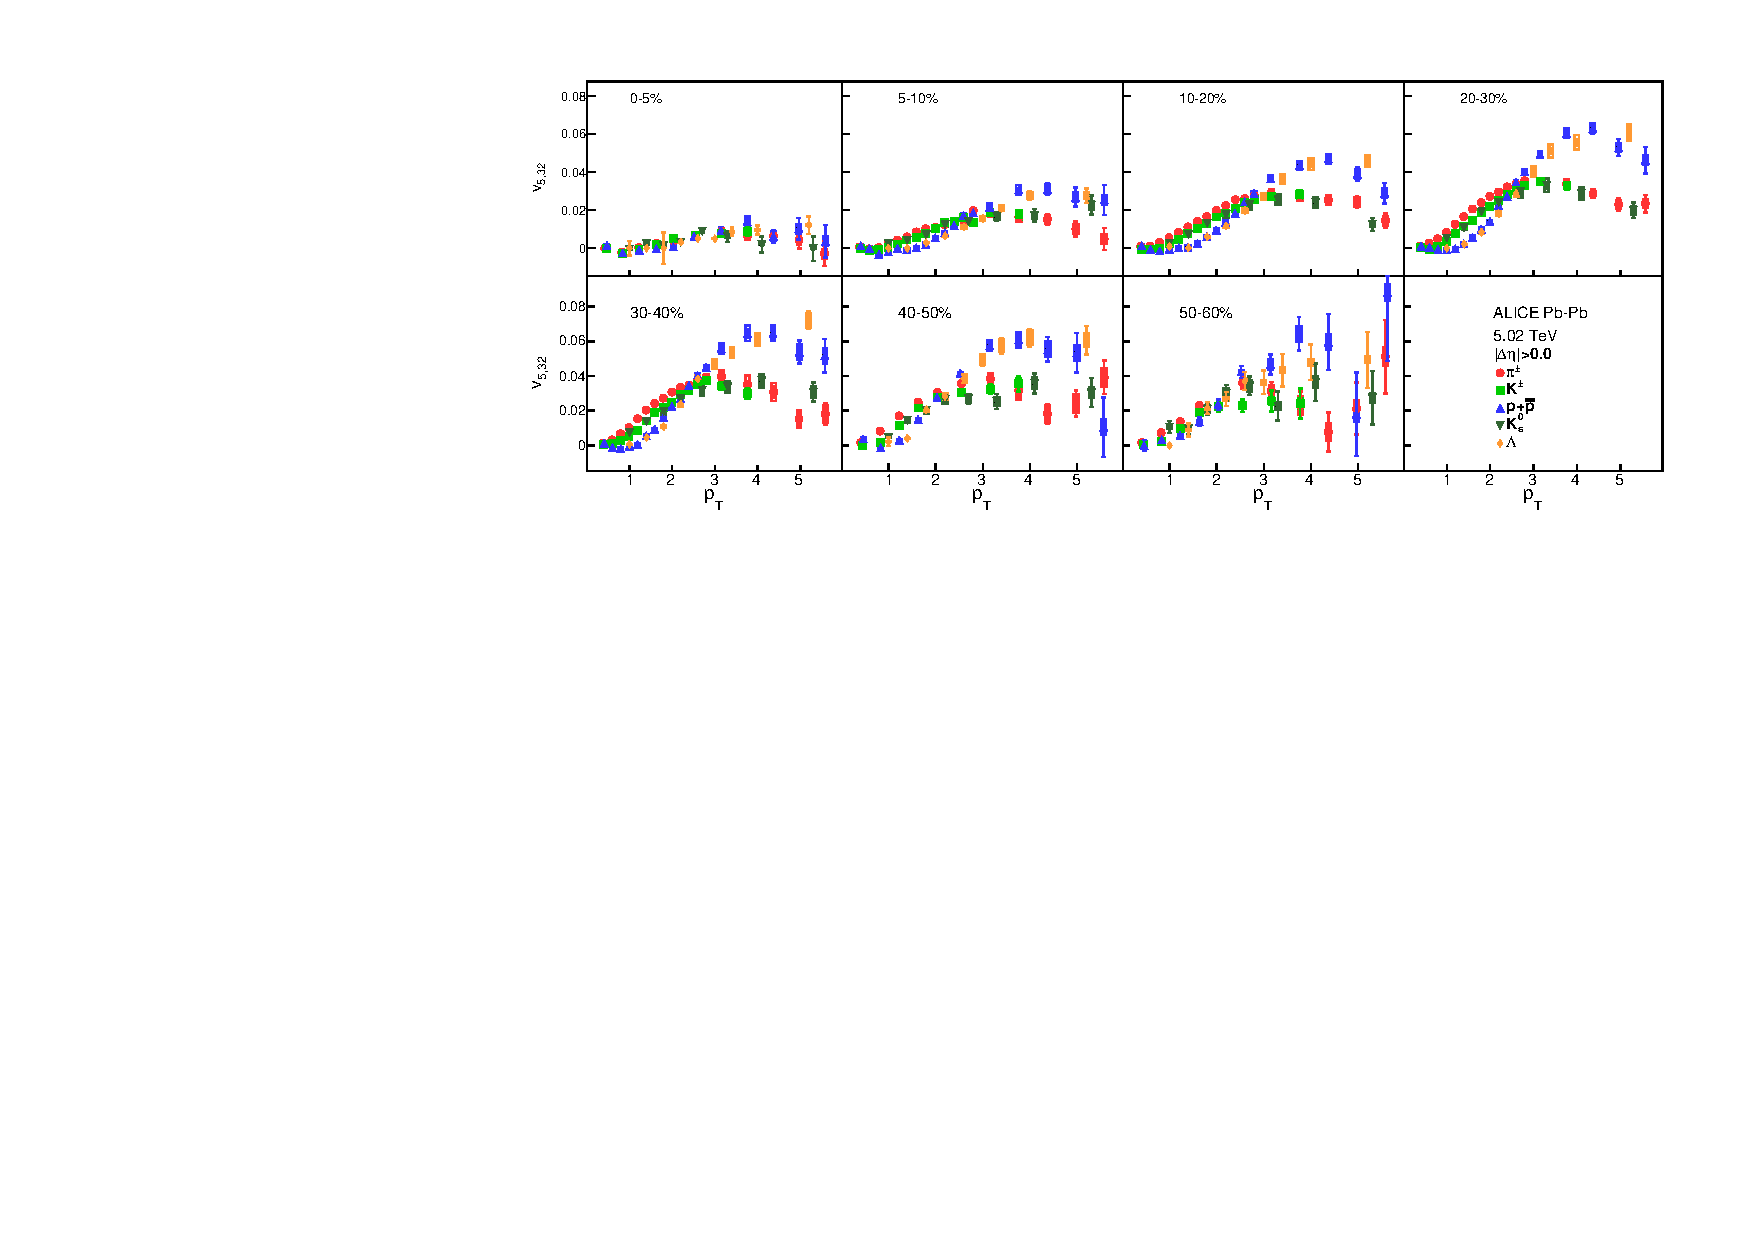
\includegraphics[scale=0.82]{figures/results/All_v523_gap00.pdf}
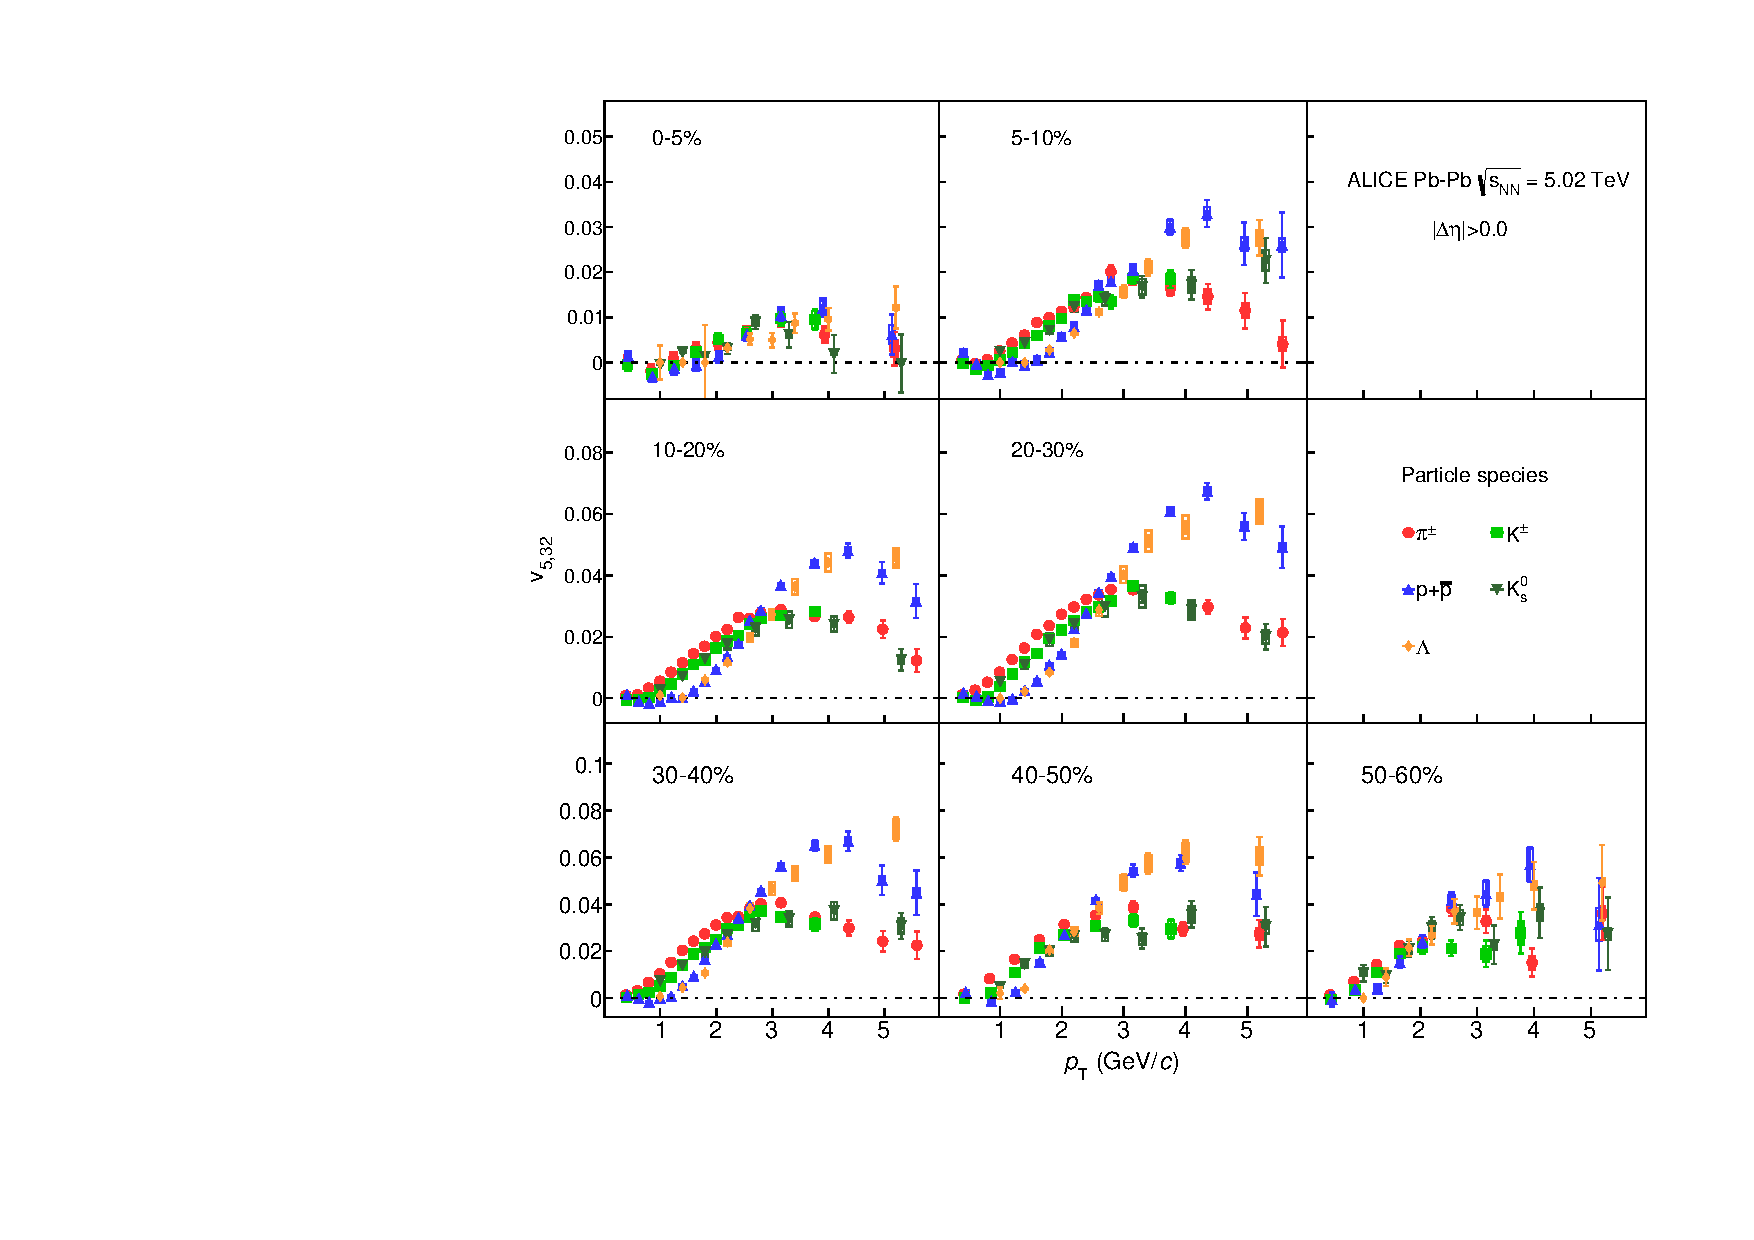
\includegraphics[scale=0.82]{figures/results/All_v523_gap00_PID2_3by3.pdf}

\end{center}
\caption{The \pT-differential $v_{5,32}$ for different particle species grouped into different centrality intervals of Pb--Pb collisions \sNN}
\label{v523_particleDependence}
\end{figure}

\begin{figure}[!htb]
\begin{center}
%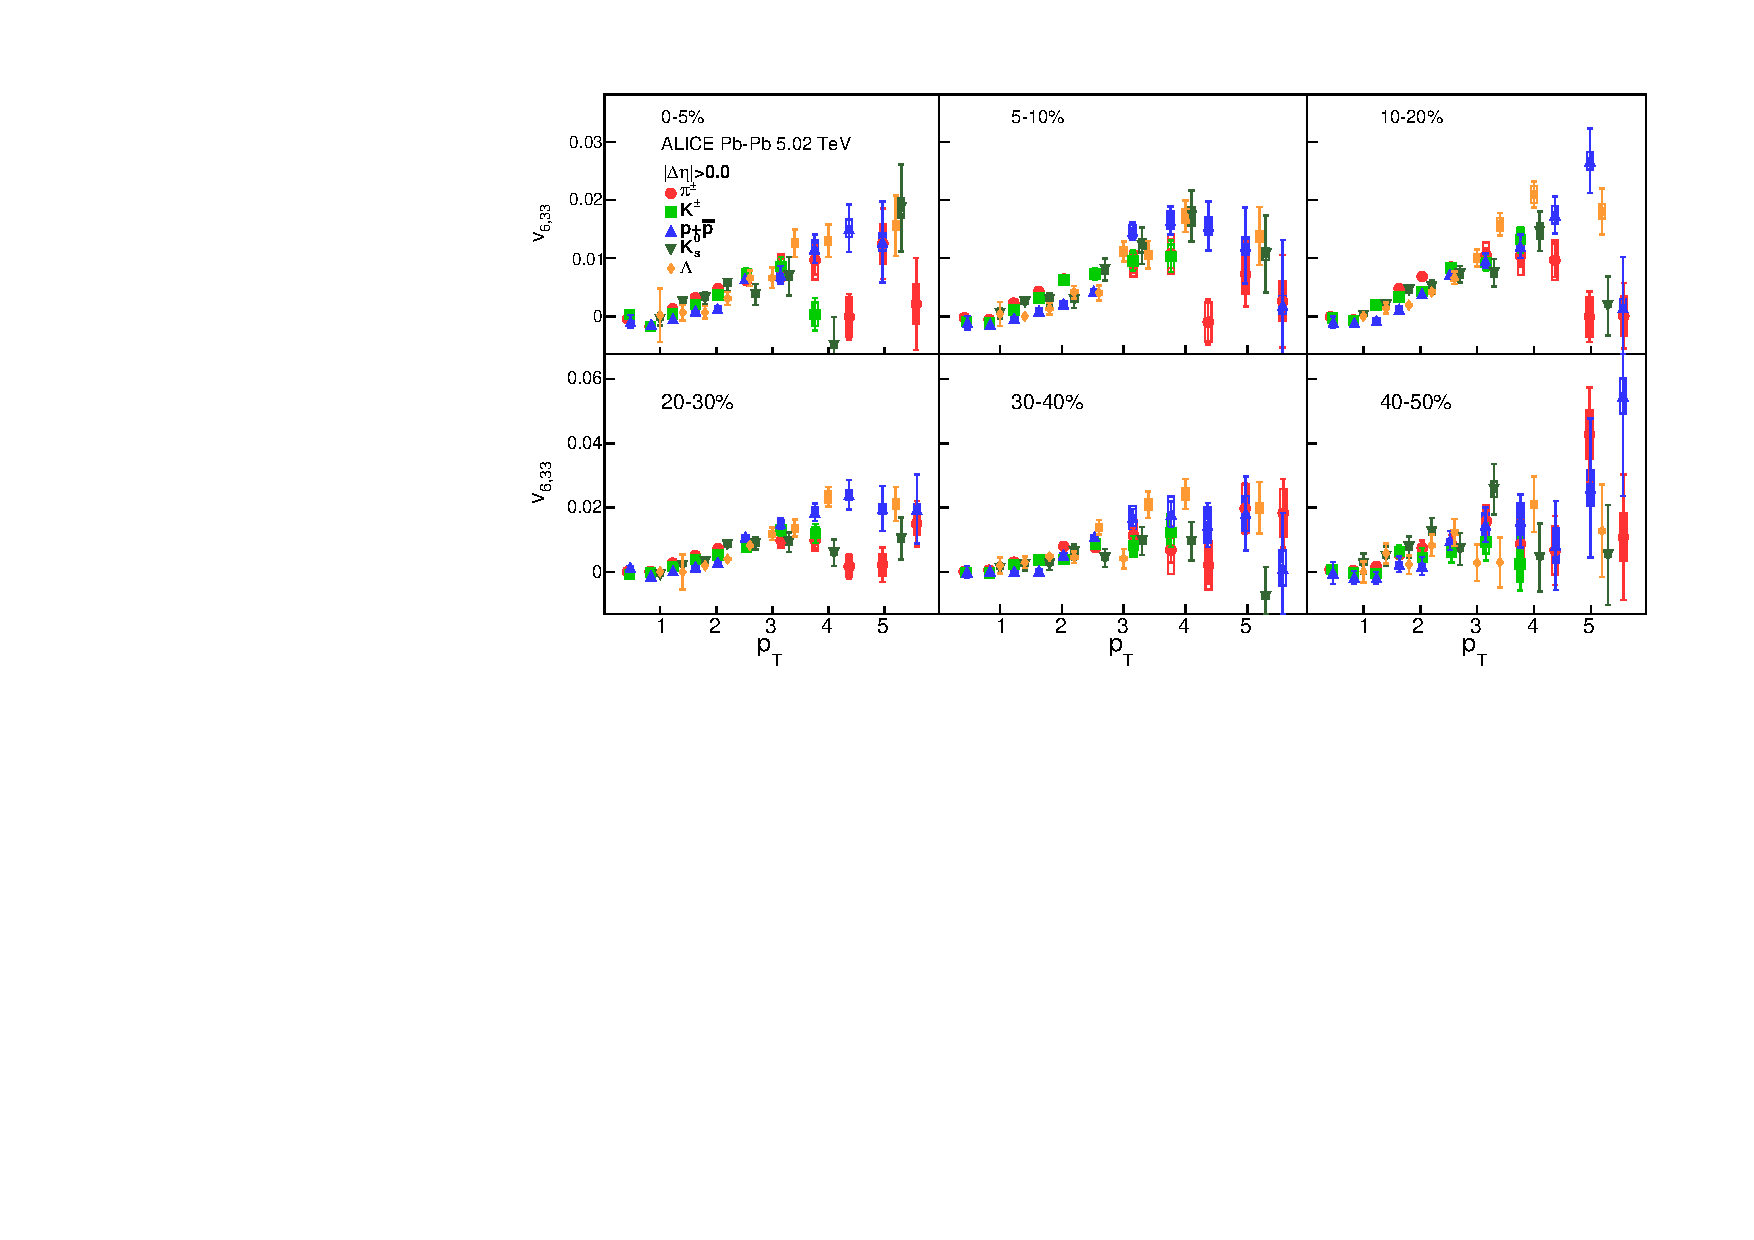
\includegraphics[scale=0.62]{figures/results/All_v633_gap00.pdf}
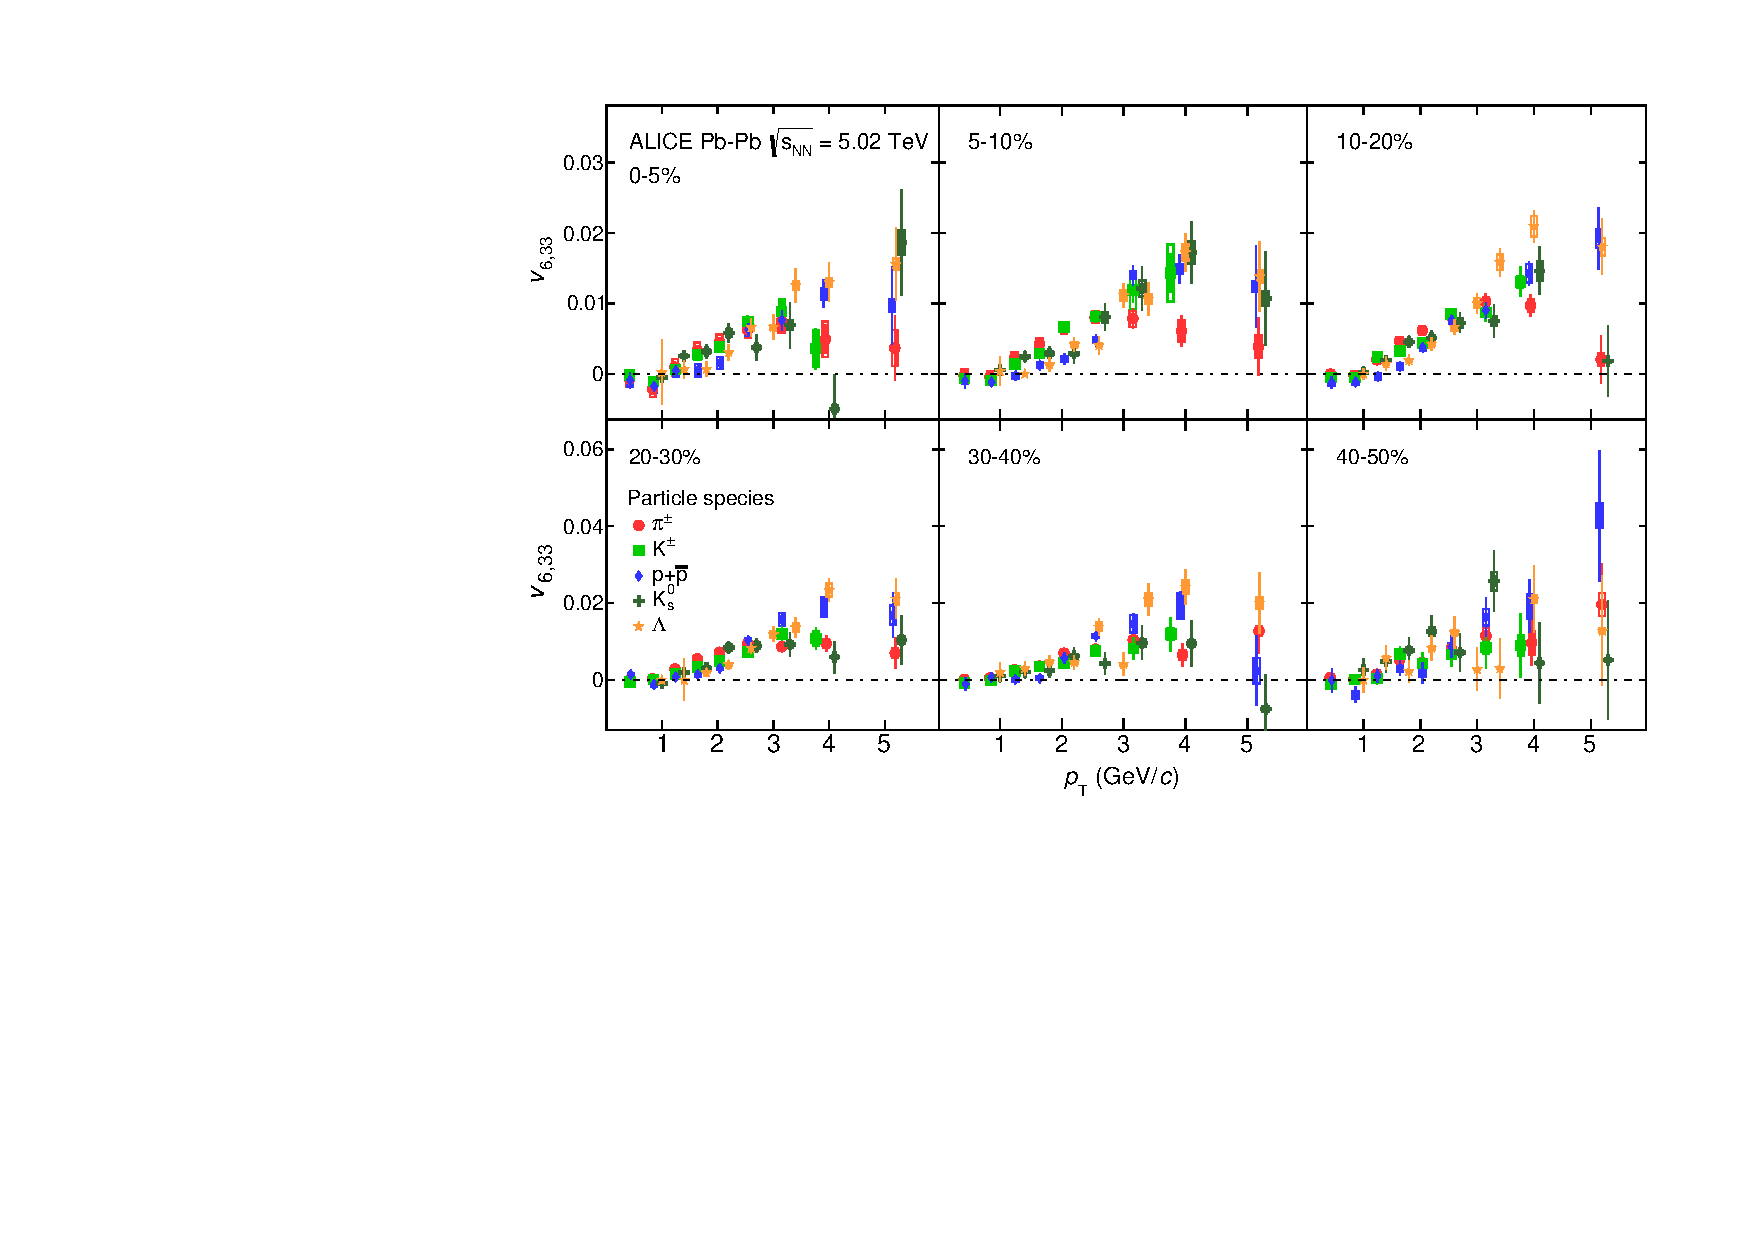
\includegraphics[scale=0.82]{figures/results/All_v633_gap00_PID2_3by2.pdf}

\end{center}
\caption{The \pT-differential $v_{6,33}$ for different particle species grouped into different centrality intervals of Pb--Pb collisions \sNN}
\label{v633_particleDependence}
\end{figure}

\begin{figure}[!htb]
\begin{center}
%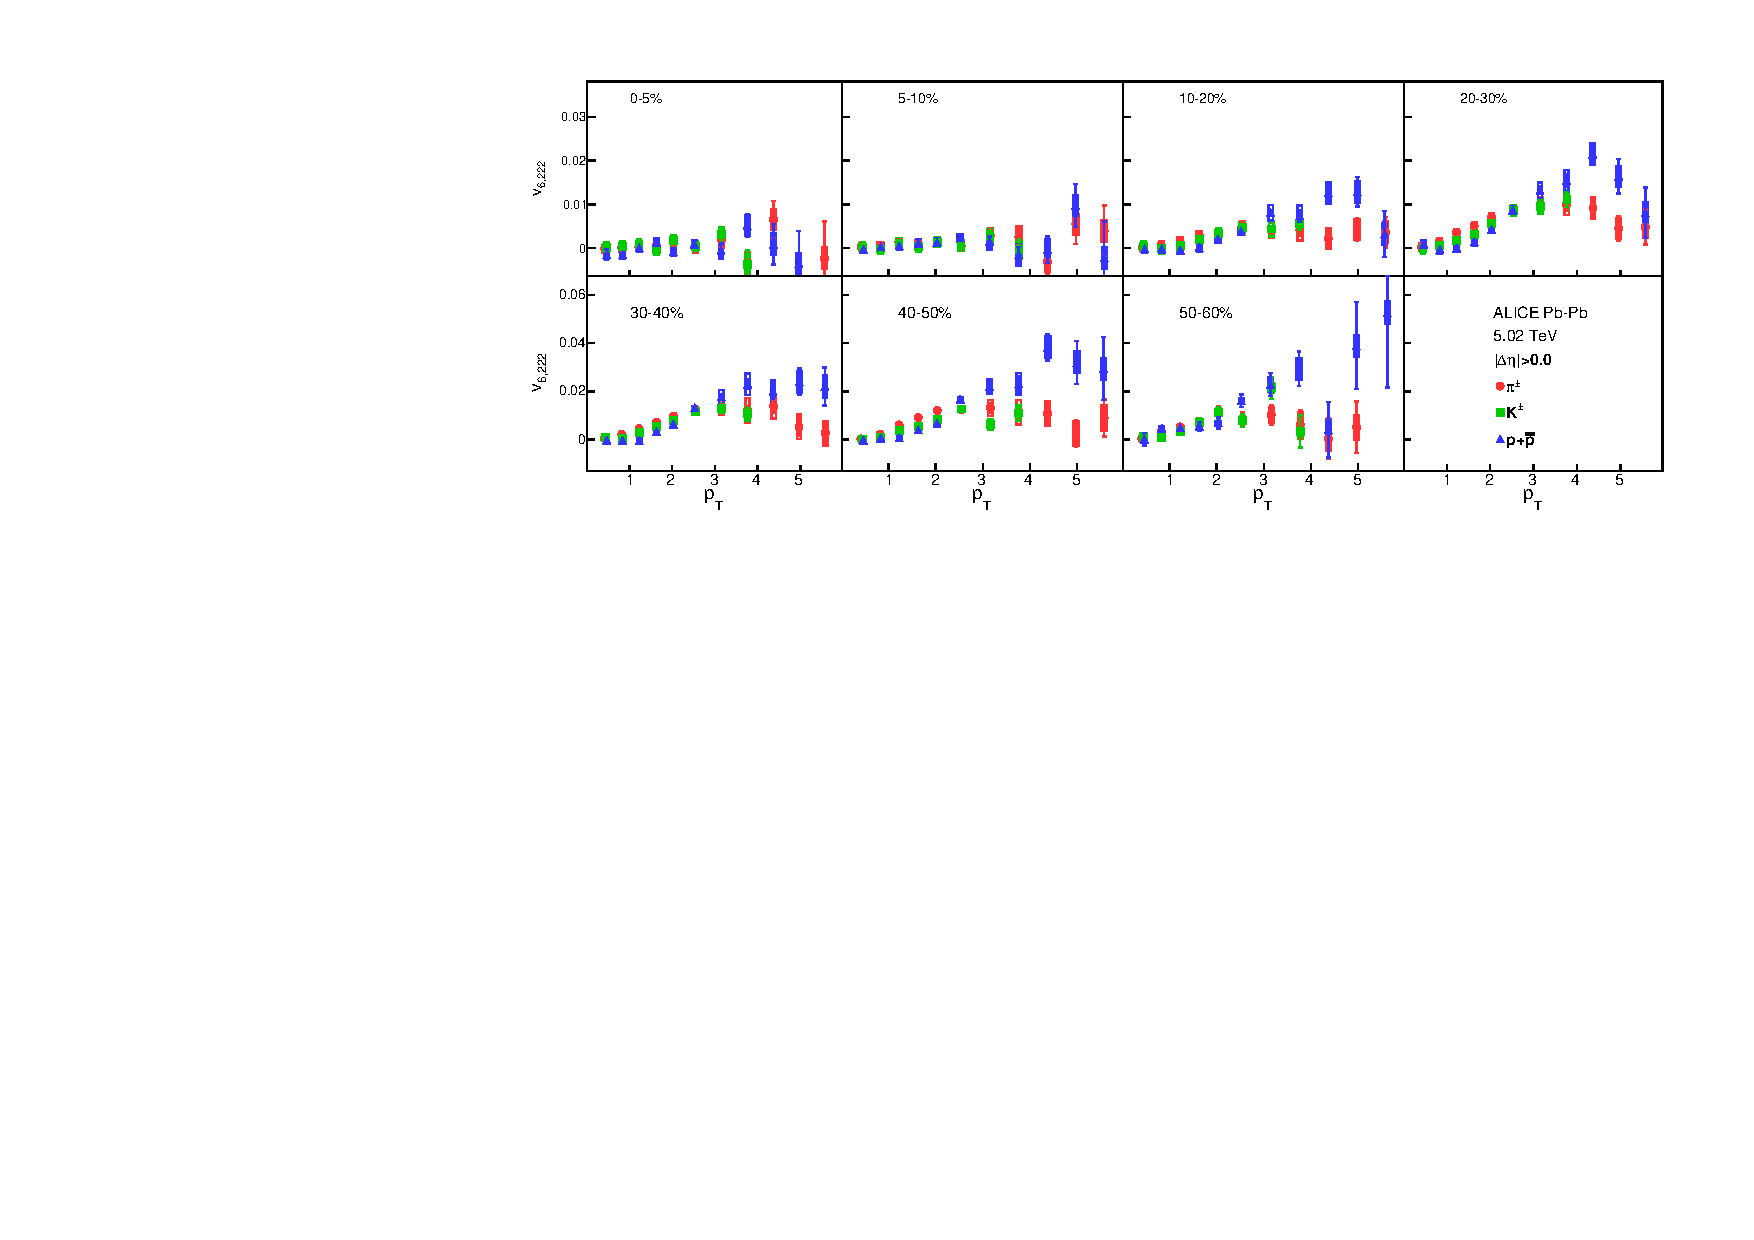
\includegraphics[scale=0.82]{figures/results/All_v6222_gap00.pdf}
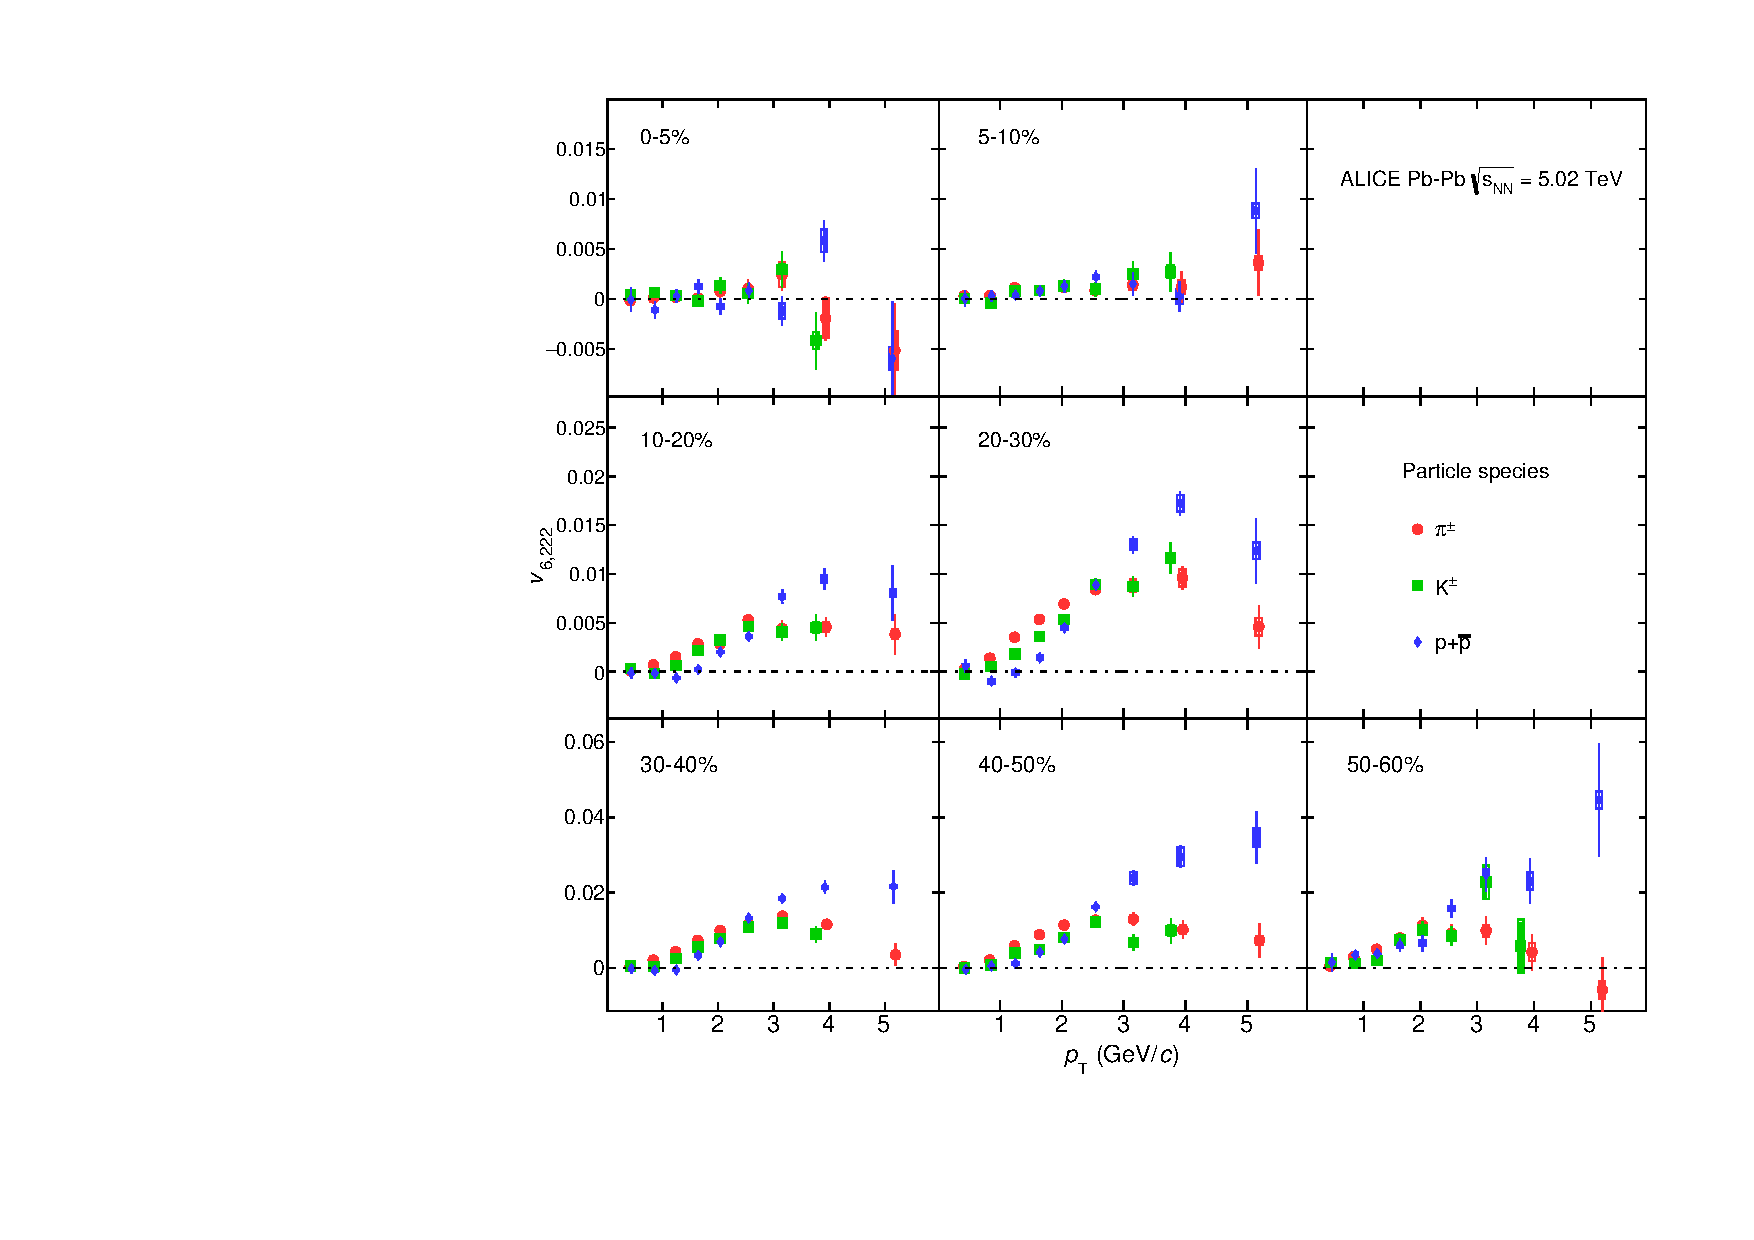
\includegraphics[scale=0.82]{figures/results/All_v6222_gap00_PID2_3by3.pdf}

\end{center}
\caption{The \pT-differential $v_{6,222}$ for different particle species grouped into different centrality intervals of Pb--Pb collisions \sNN}
\label{v6222_particleDependence}
\end{figure}

\newpage

In addition, in the intermediate \pT~region (for \pT $> 2.5$ \GeV) the data points of Figs. \ref{v422_particleDependence}-\ref{v6222_particleDependence} exhibit a particle type grouping. In particular, $v_{n,mk}$ of mesons (\pion, \kaon, \Ks~and $\phi$) and baryons (\proton~and \lambdas) group based on their type, with $v_{n,mk}$ of baryons having a larger magnitude. This particle type grouping was previously observed in the anisotropic flow measurements of various particle species \cite{Abelev:2014pua,Adam:2016nfo,Acharya:2018zuq,Adams:2003am,Abelev:2007qg,Adler:2003kt,Adare:2006ti}. This suggests that flow develops at the partonic stage and if so, combining two or three quarks to form hadronic states might result into hadrons inheriting the transverse momentum and subsequently, $v_{n}$ of their constituents. As a next step it was suggested to use a form of number of constituent quark (NCQ) scaling in which both flow coefficients and \pT~were scaled by the number of constituent quarks ($n_{q}$). This scaling, worked initially at RHIC energies, although later measurements revealed sizeable deviations from a perfect scaling \cite{Adams:2003am,Abelev:2007qg,Adler:2003kt,Adare:2006ti}. ALICE measurements showed that the NCQ scaling at LHC energies holds at an approximate level of 20\% for $v_{n}$ \cite{Abelev:2014pua,Adam:2016nfo,Acharya:2018zuq}. Various theoretical ideas were created to address the origin of possible scaling by requiring quark coalescence to be the dominant particle production mechanism in the intermediate \pT~region, where the hydrodynamic evolution of the fireball is not the driving force behind the development of anisotropic flow \cite{Voloshin:2002wa,Molnar:2003ff}.

%\subsection{Test of scaling properties}
%\label{subsection:NCQscaling}

Figures \ref{v422_NCQ}, \ref{v523_NCQ}, \ref{v633_NCQ} and \ref{v6222_NCQ} present $v_{4,22}$, $v_{5,32}$, $v_{6,33}$ and $v_{6,222}$ respectively, scaled by the inverse of number of constituent quarks ($n_{q}$) as a function of \pTnq~for \pion, \kaon, \Ks, \proton, \lambdas~and $\phi$-meson grouped in different centrality intervals. The scaling is consistent with the observations reported for higher order anisotropic flow coefficients \cite{Acharya:2018zuq}. Similarly, for non-linear flow modes this scaling hold at an approximate level ($\pm$20\%). 

\begin{figure}[!htb]
\begin{center}
%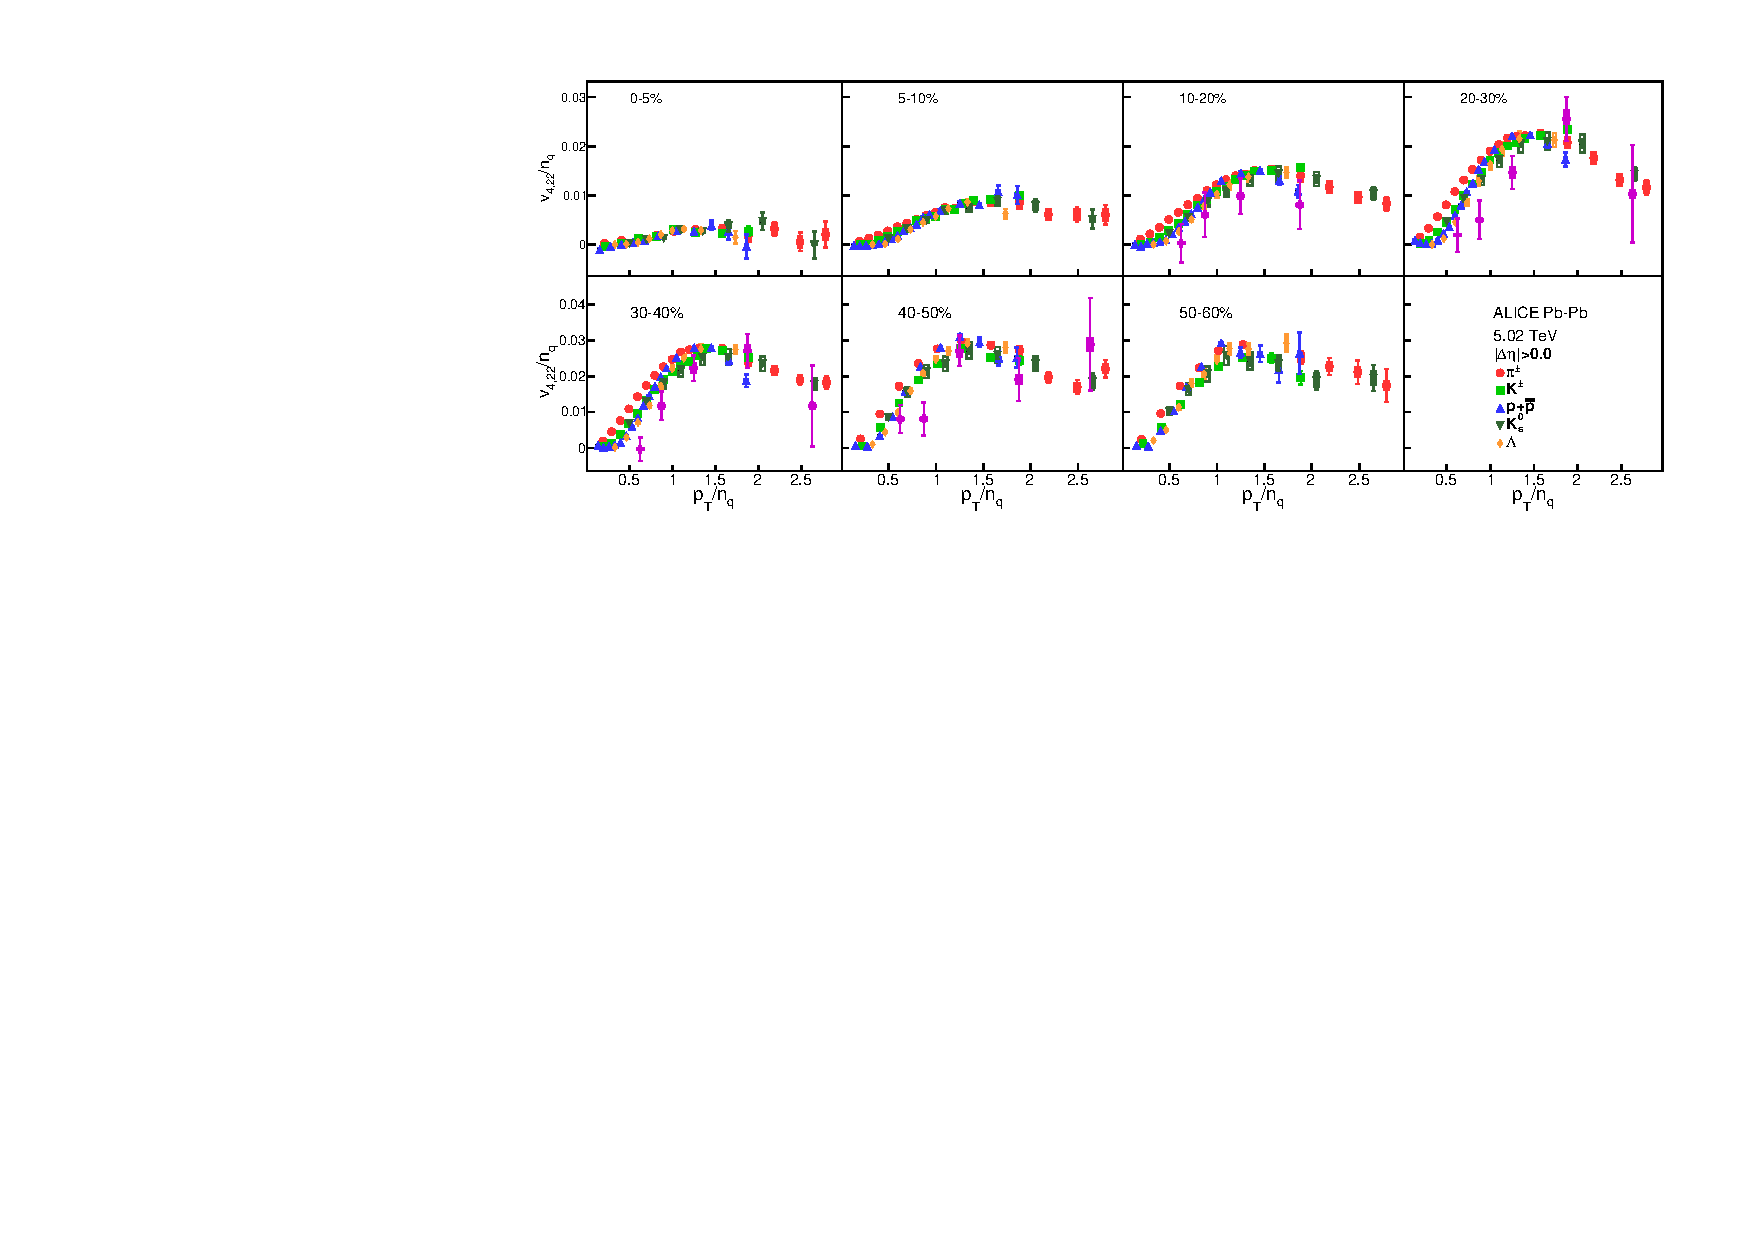
\includegraphics[scale=0.82]{figures/scaling/All_v422_gap00_NCQ.pdf}
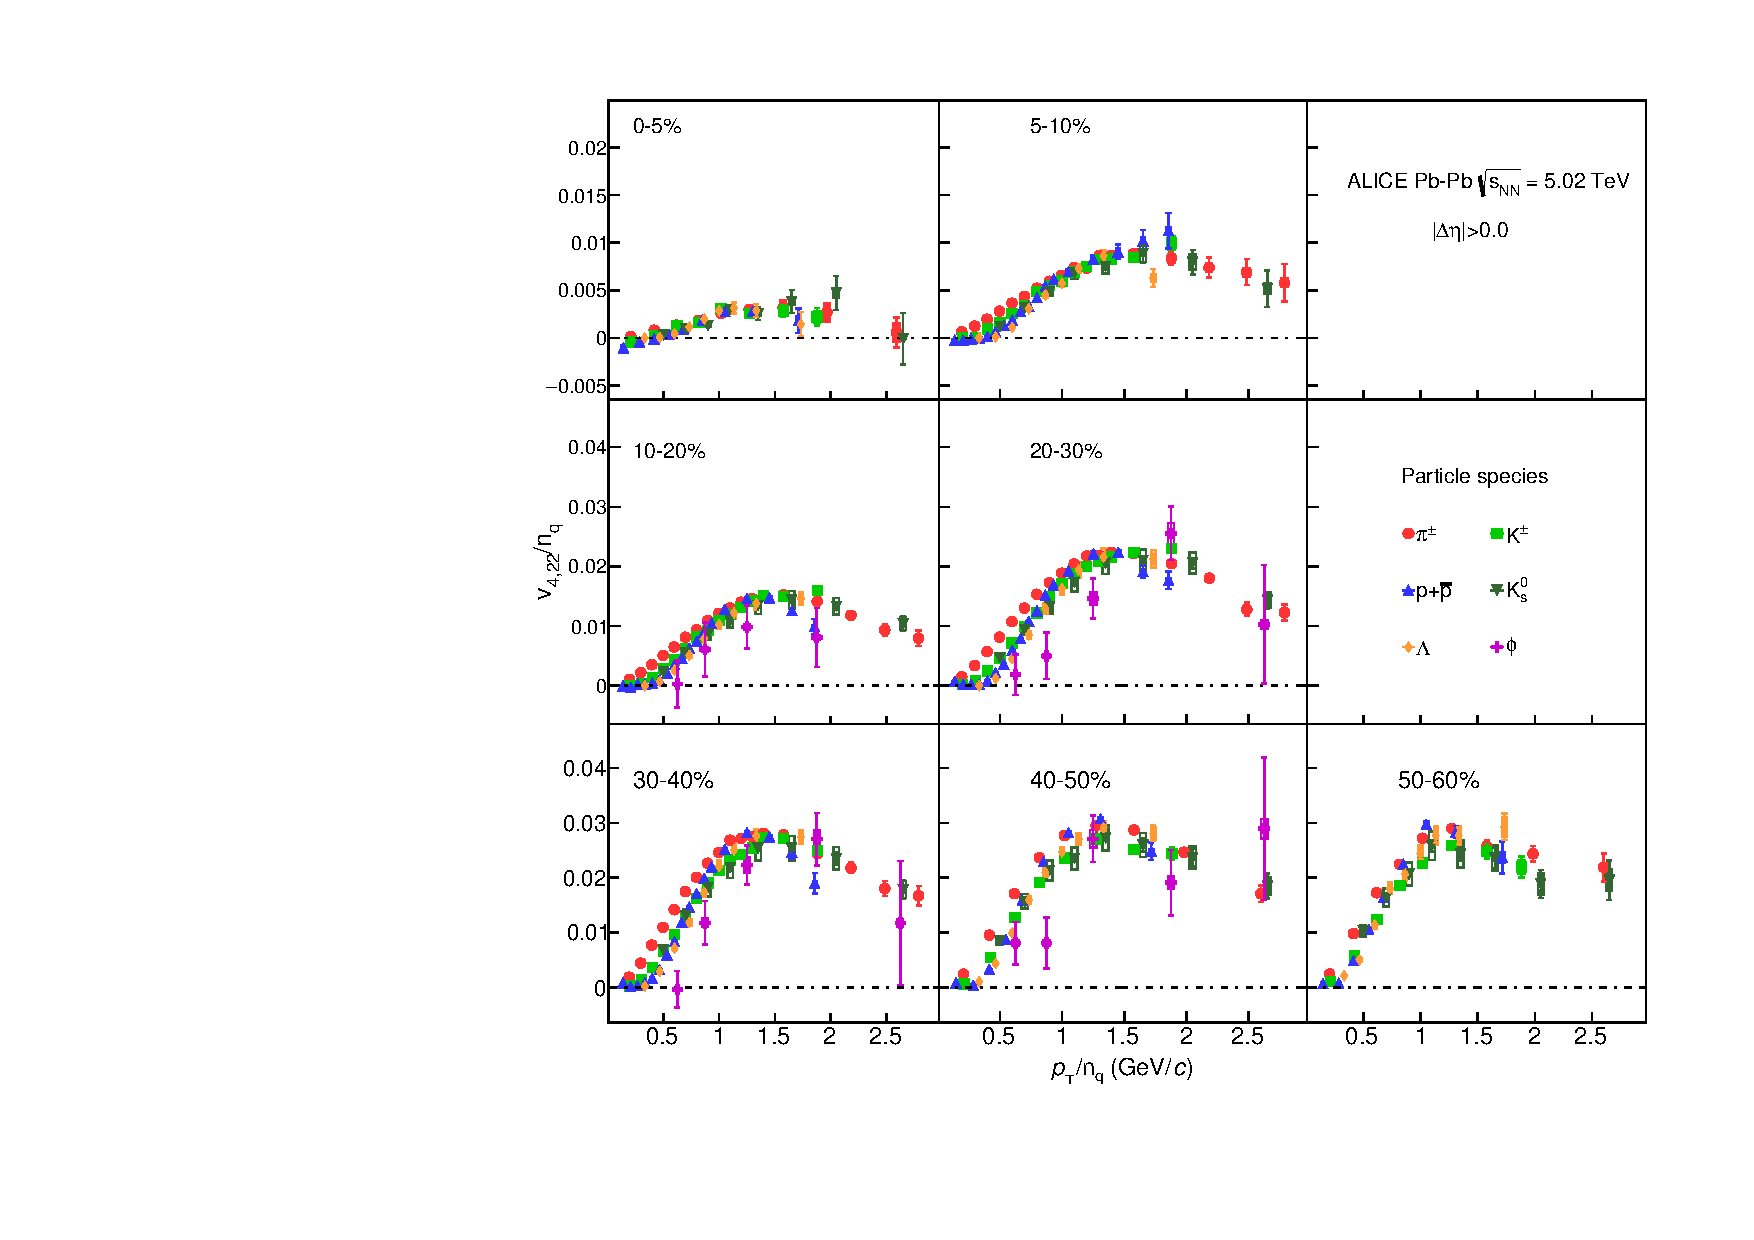
\includegraphics[scale=0.82]{figures/scaling/All_v422_gap00_NCQ_3by3.pdf}
\end{center}
\caption{The $p_{\rm{T}}/n_{q}$-dependence of $v_{4,22}/n_{q}$ for different particle species grouped into different centrality intervals of Pb--Pb collisions \sNN}
\label{v422_NCQ}
\end{figure}

\begin{figure}[!htb]
\begin{center}
%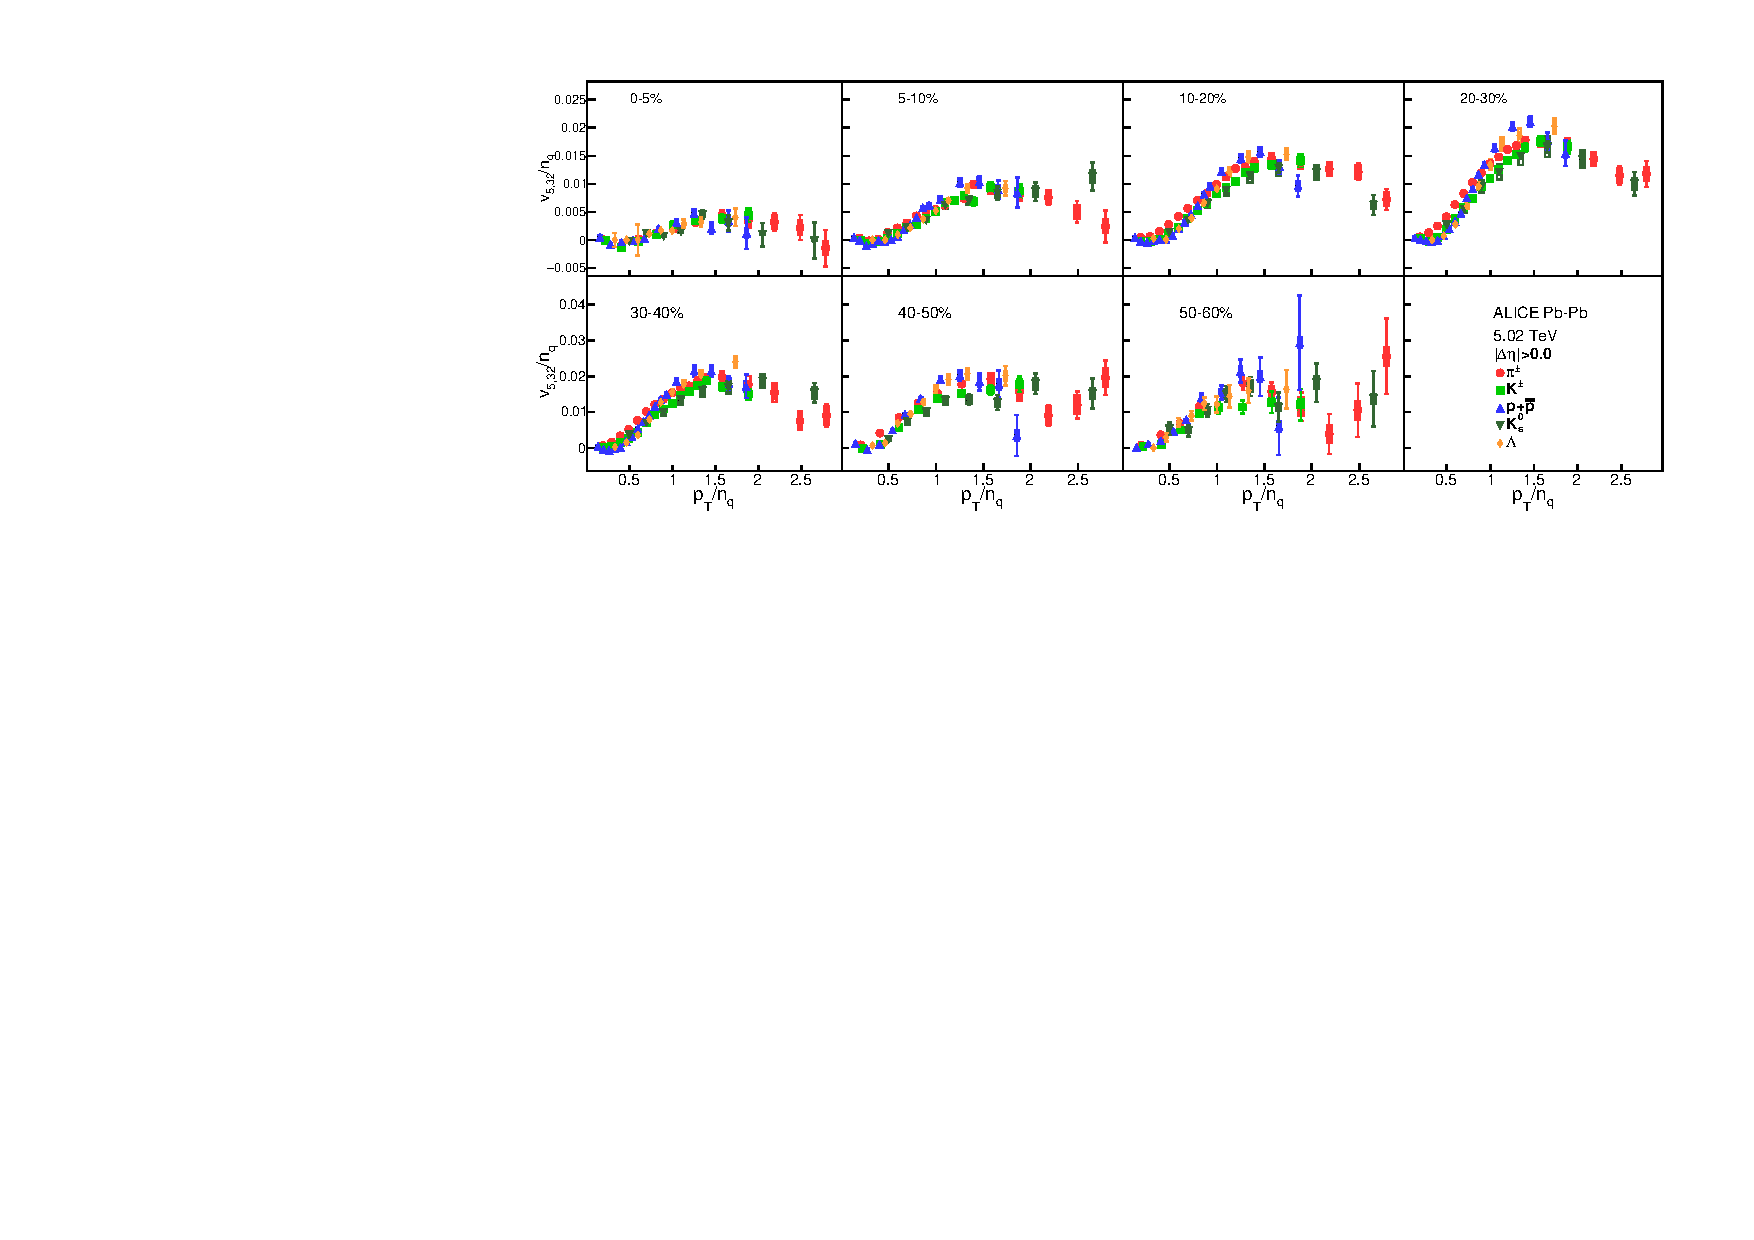
\includegraphics[scale=0.82]{figures/scaling/All_v523_gap00_NCQ.pdf}
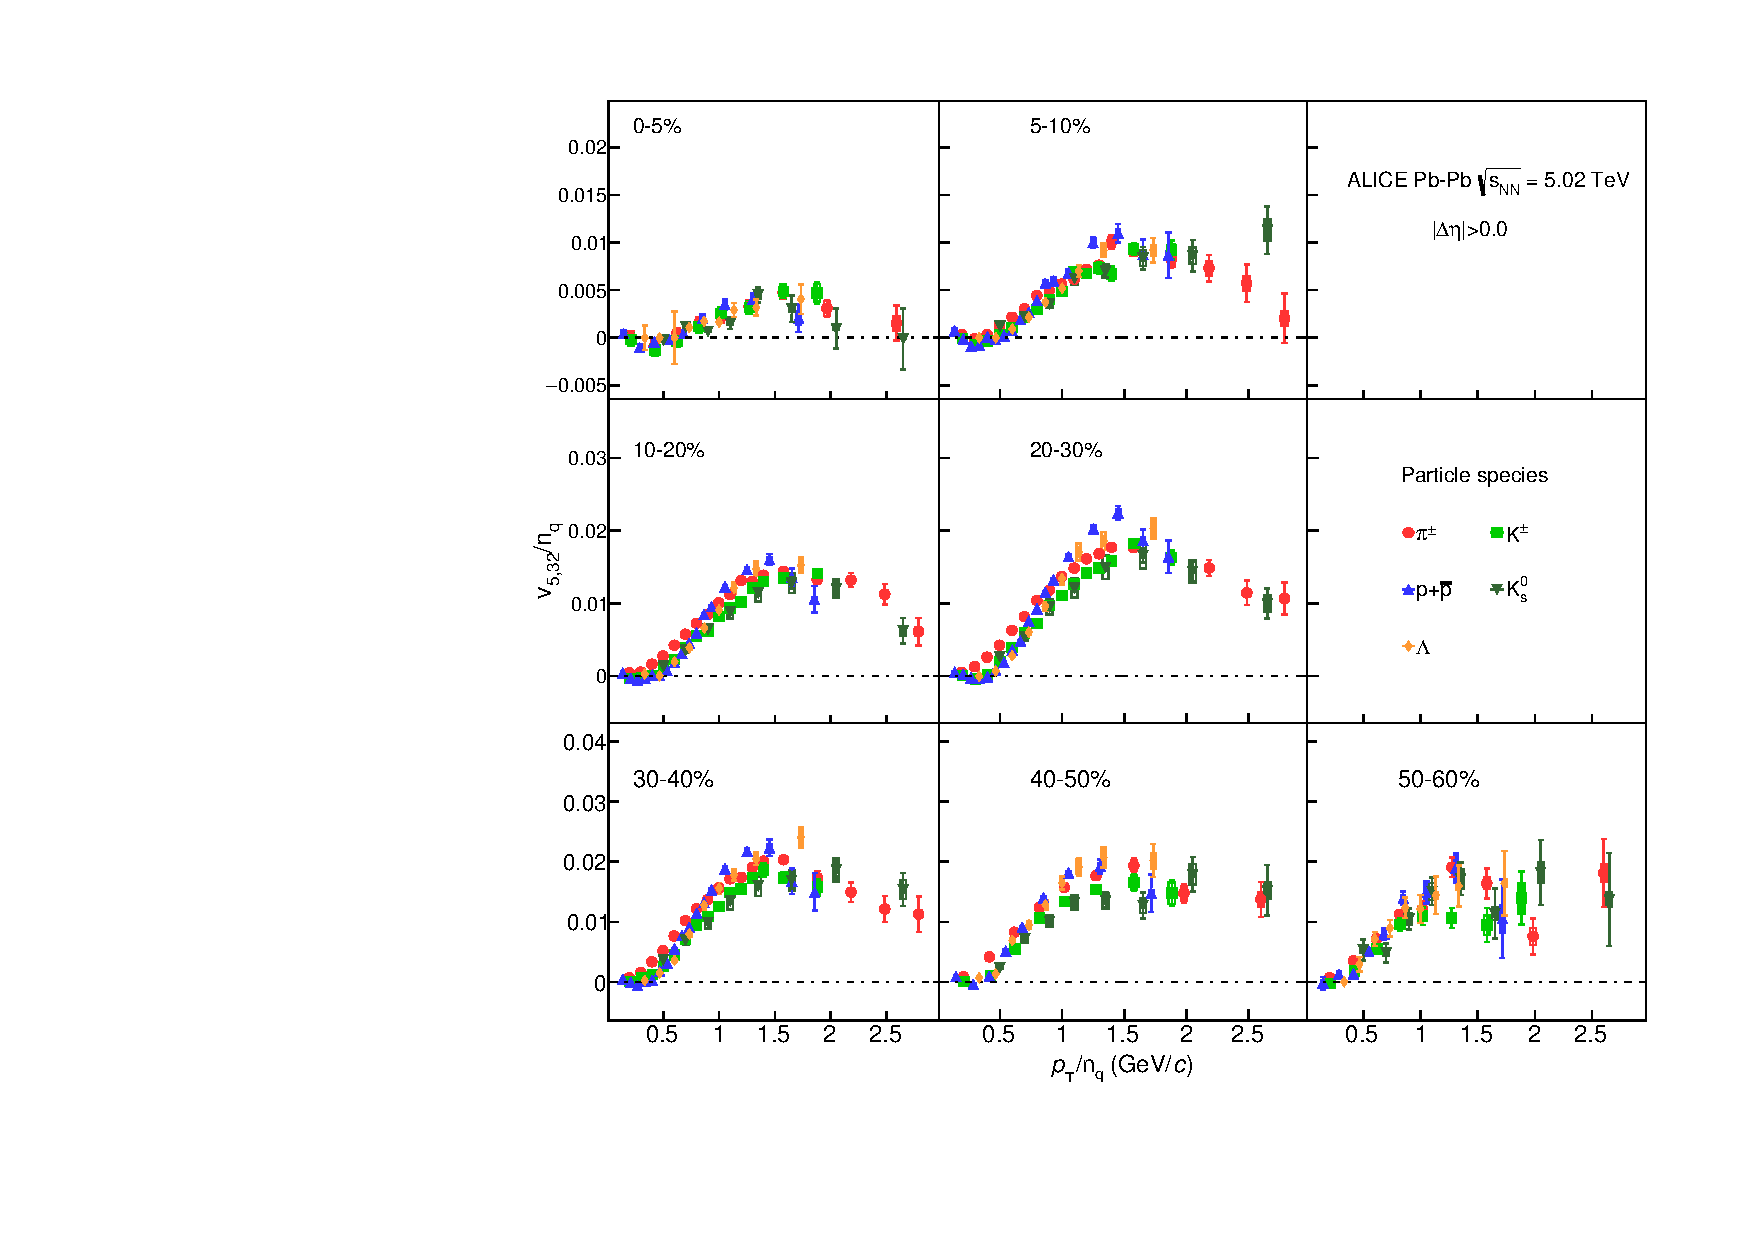
\includegraphics[scale=0.82]{figures/scaling/All_v523_gap00_NCQ_3by3.pdf}

\end{center}
\caption{The $p_{\rm{T}}/n_{q}$-dependence of $v_{5,32}/n_{q}$ for different particle species grouped into different centrality intervals of Pb--Pb collisions \sNN}
\label{v523_NCQ}
\end{figure}

\begin{figure}[!htb]
\begin{center}
%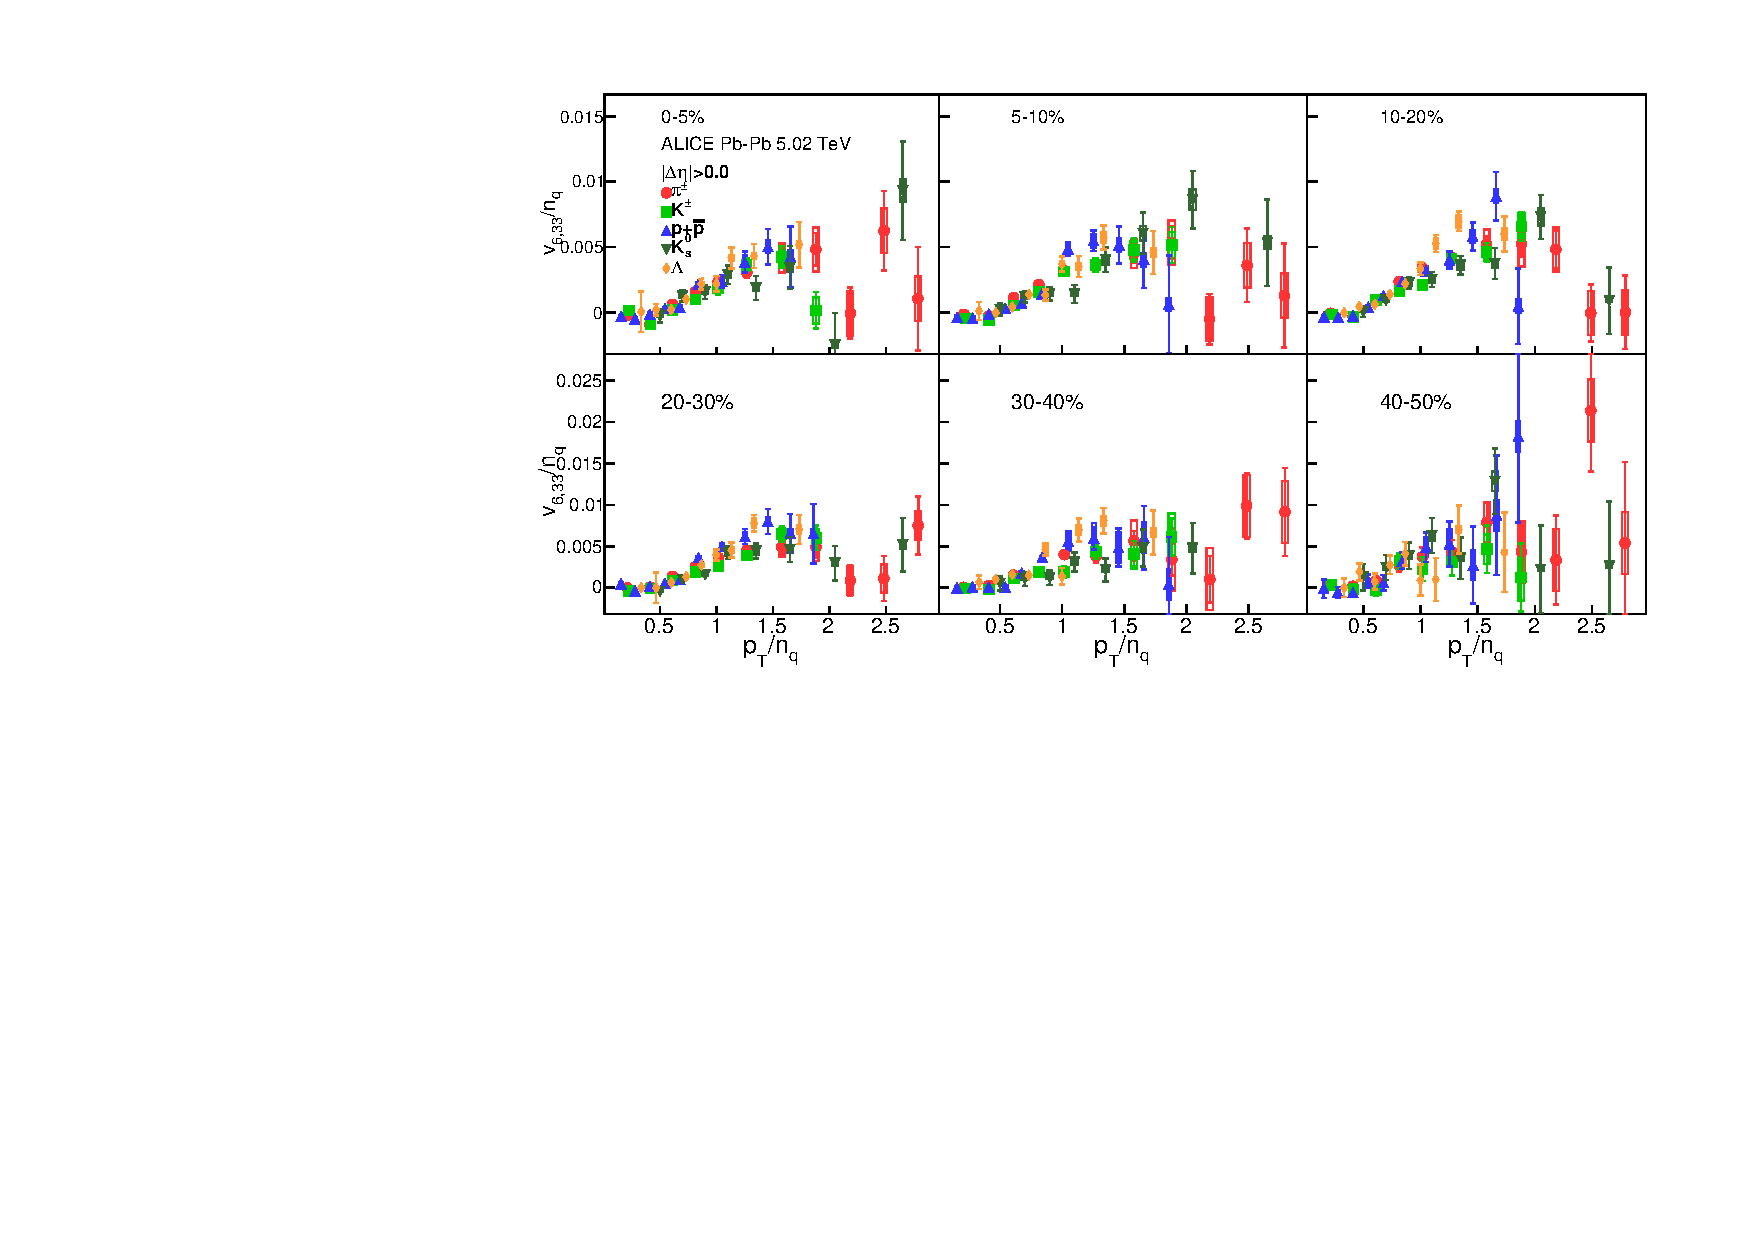
\includegraphics[scale=0.82]{figures/scaling/All_v633_gap00_NCQ.pdf}
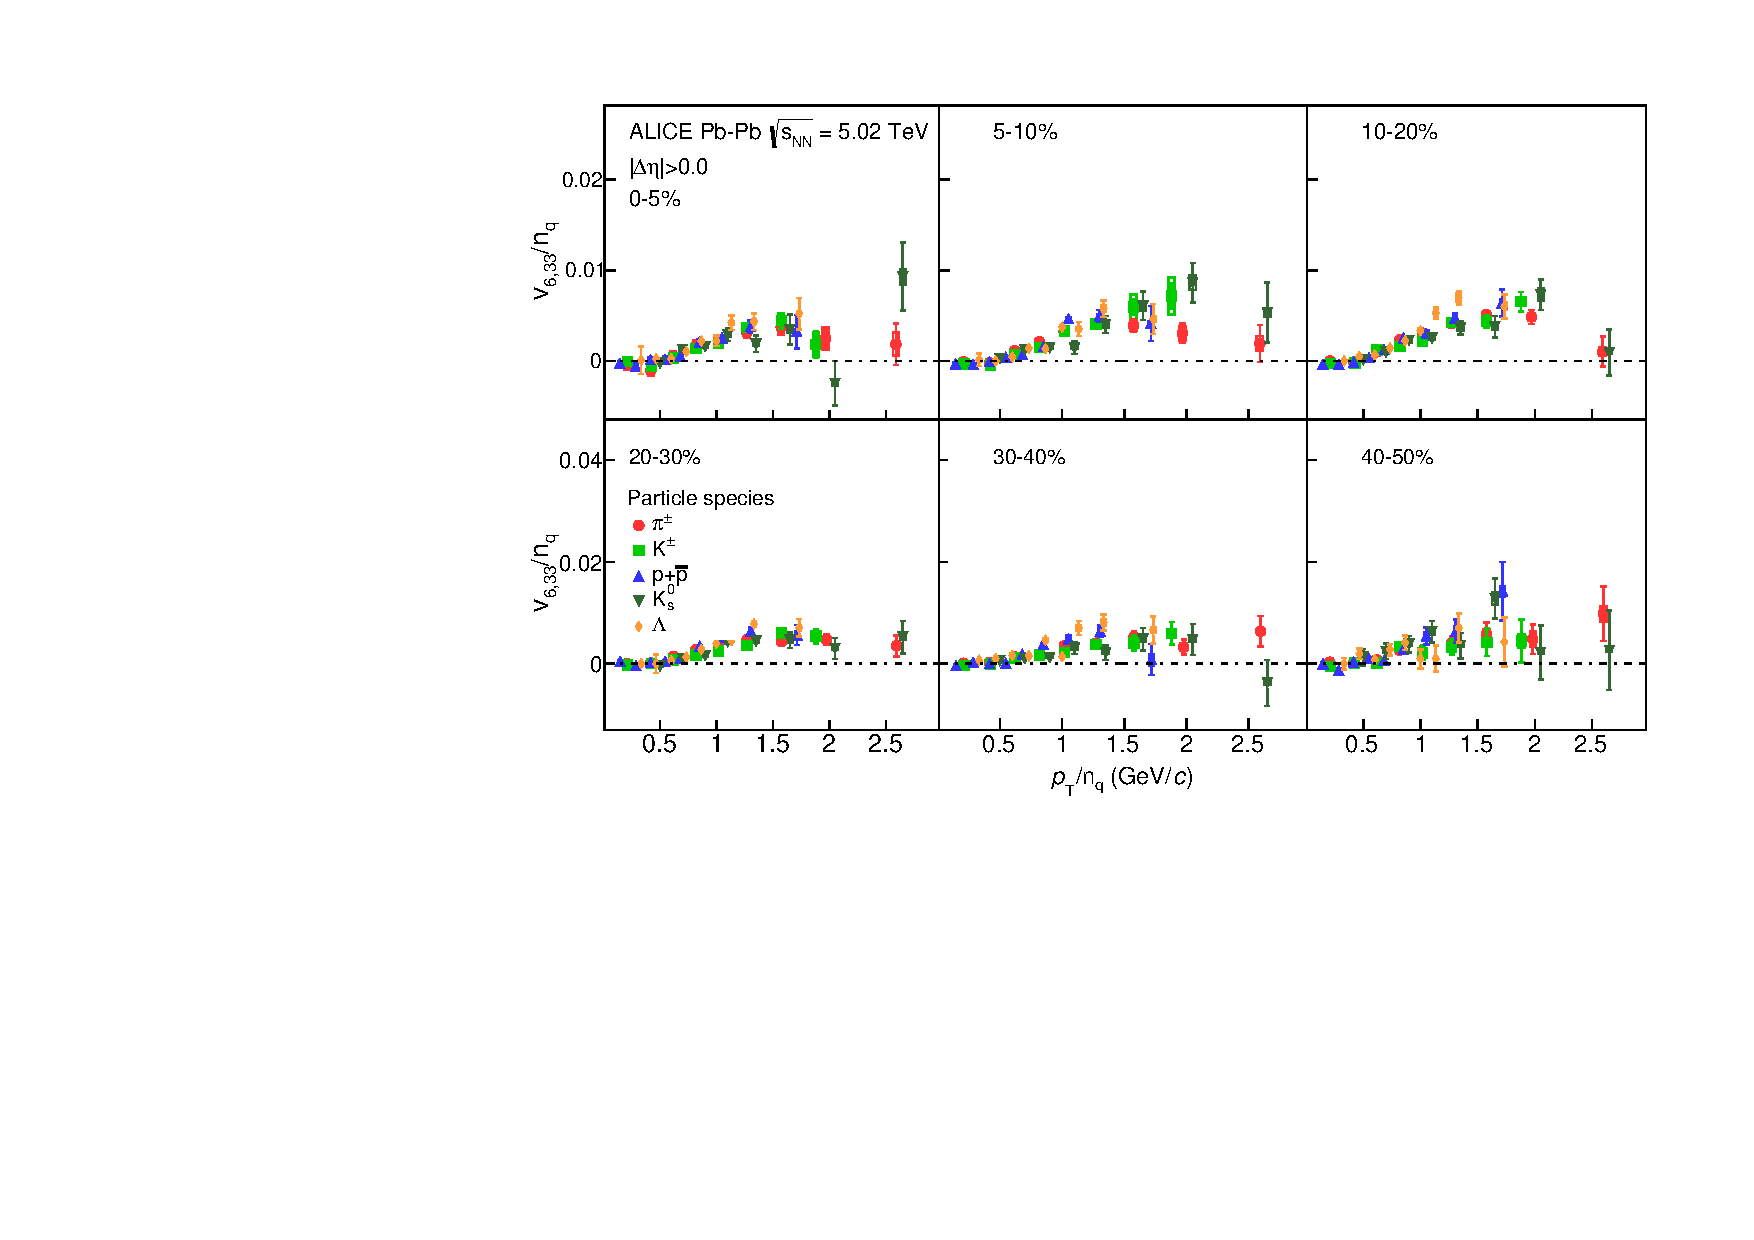
\includegraphics[scale=0.82]{figures/scaling/All_v633_gap00_NCQ_3by2.pdf}
\end{center}
\caption{The $p_{\rm{T}}/n_{q}$-dependence of $v_{6,33}/n_{q}$ for different particle species grouped into different centrality intervals of Pb--Pb collisions \sNN}
\label{v633_NCQ}
\end{figure}

\begin{figure}[!htb]
\begin{center}
%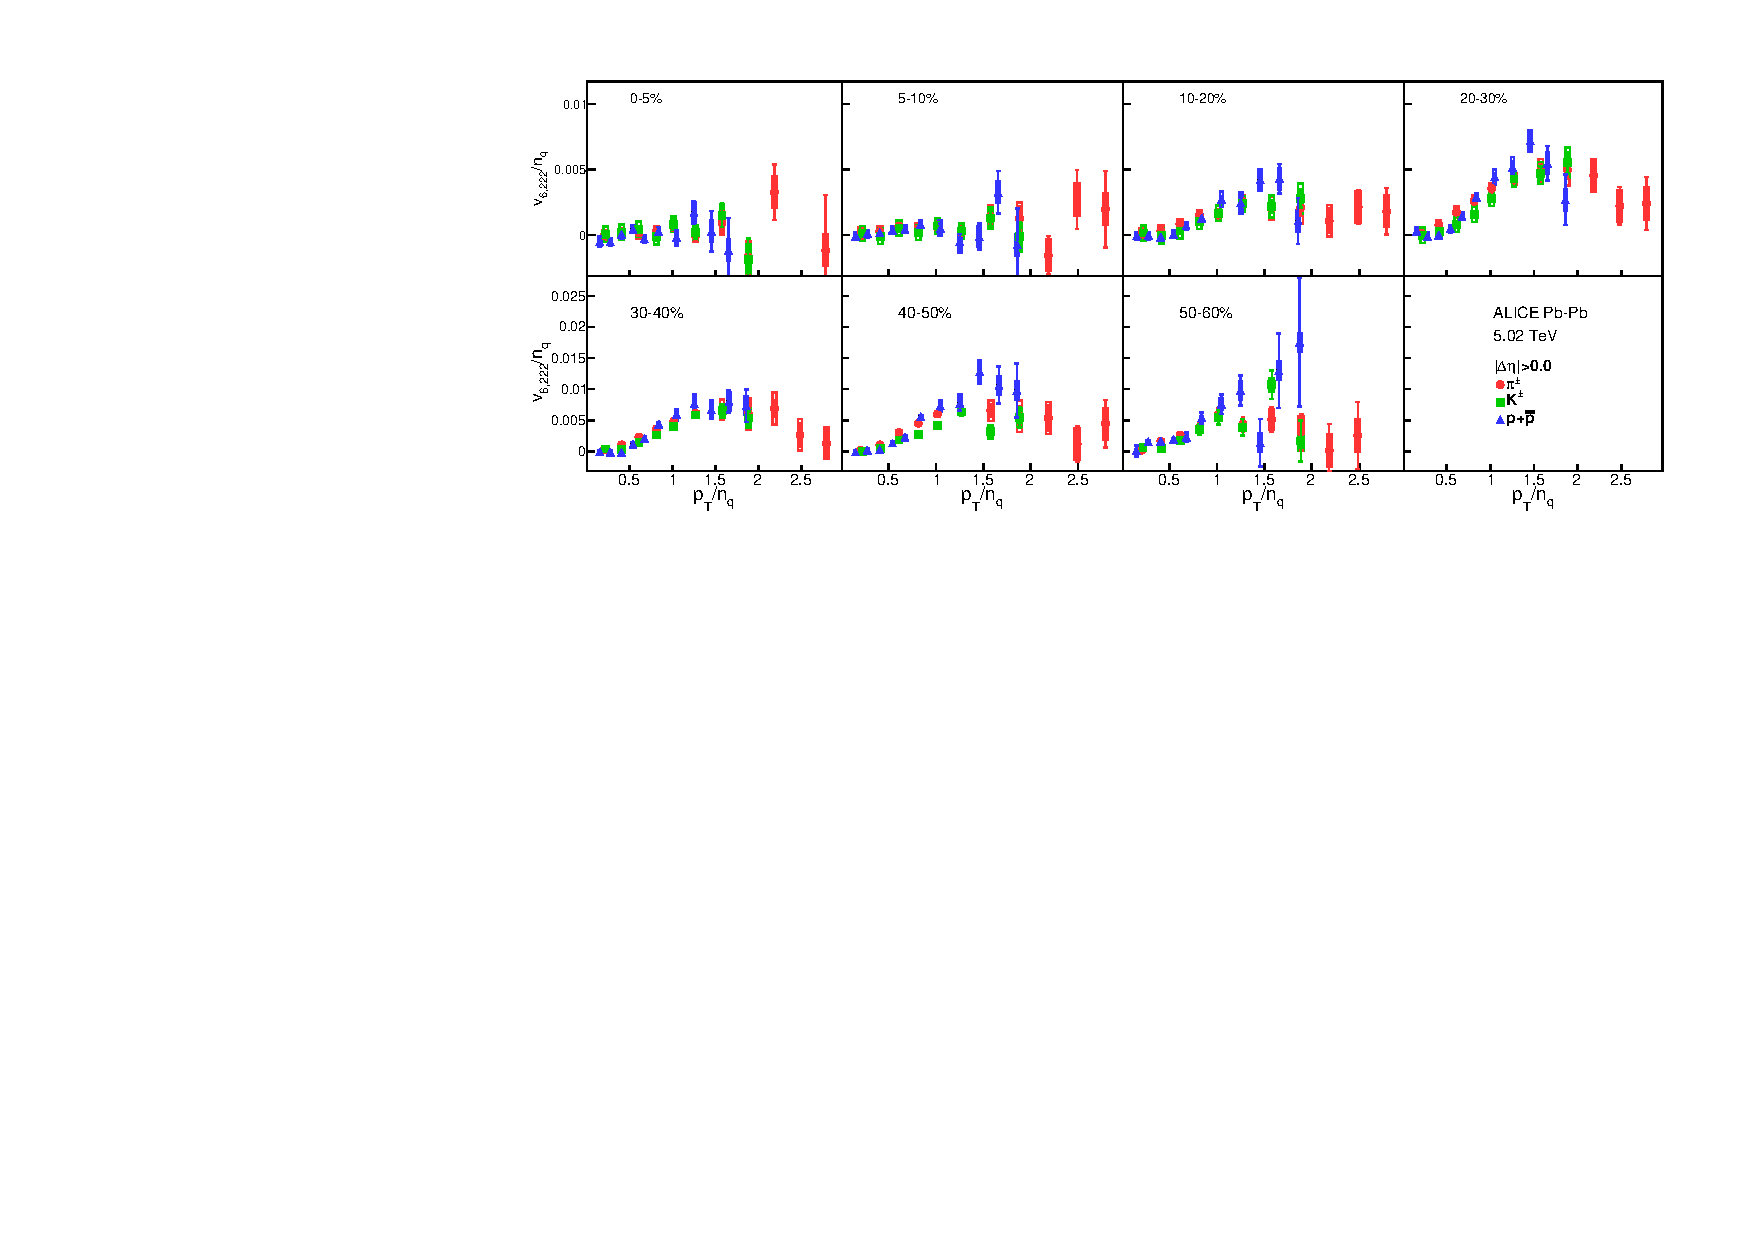
\includegraphics[scale=0.82]{figures/scaling/All_v6222_gap00_NCQ.pdf}
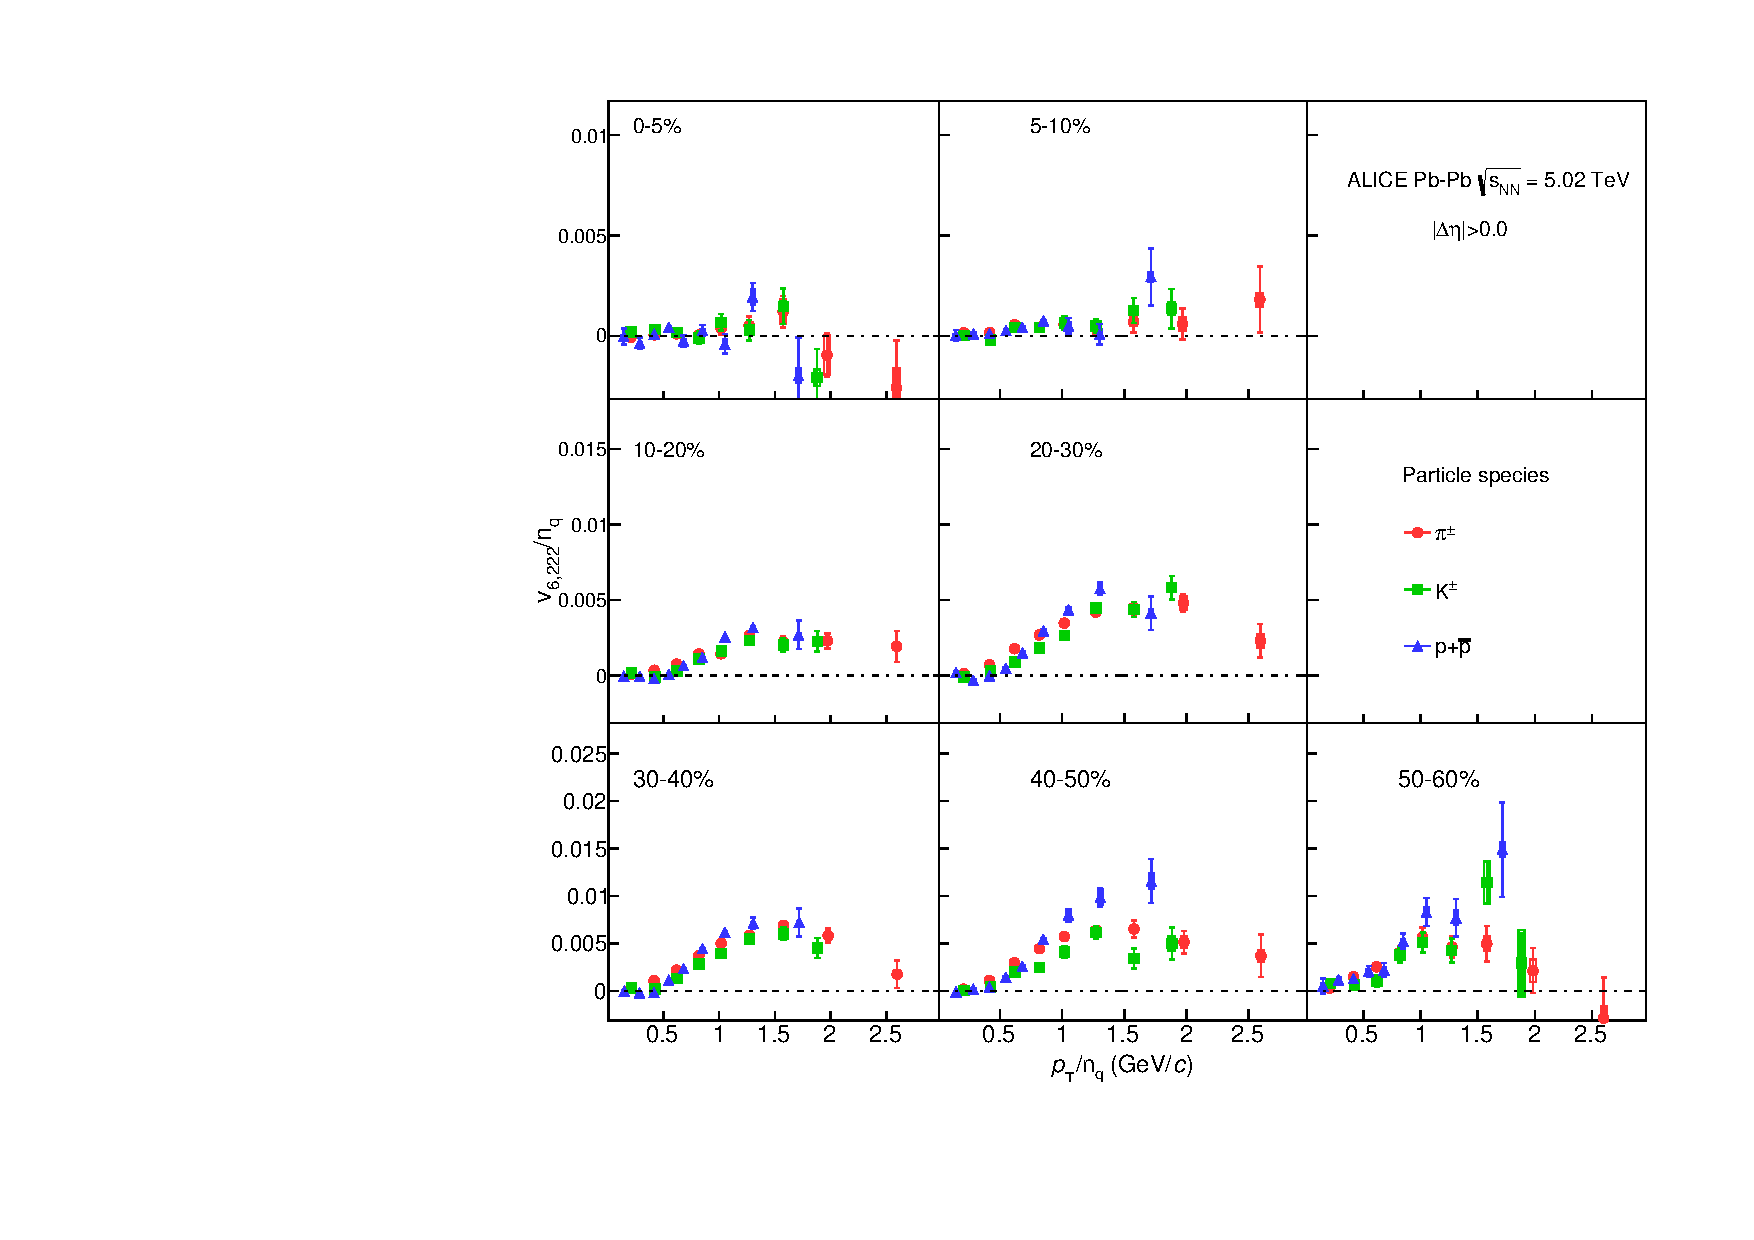
\includegraphics[scale=0.82]{figures/scaling/All_v6222_gap00_NCQ_3by3.pdf}

\end{center}
\caption{The $p_{\rm{T}}/n_{q}$-dependence of $v_{6,222}/n_{q}$ for different particle species grouped into different centrality intervals of Pb--Pb collisions \sNN}
\label{v6222_NCQ}
\end{figure}



\newpage
\subsection{Comparison with models}
\label{SubSec:hydro}
%Measurements of anisotropic flow coefficients, $v_{n}$, at RHIC and the LHC are described well by hydrodynamic calculations \cite{Xu:2016hmp, McDonald:2016vlt, Zhao:2017yhj}. 

The comparisons of the anisotropic flow measurements and hydrodynamic calculations have been presented and discussed in great details in \cite{Xu:2016hmp, McDonald:2016vlt, Zhao:2017yhj}. A recent comparison between $v_{n}$ measurements at ALICE \cite{Acharya:2018zuq} and two hydrodynamic calculations from \cite{Zhao:2017yhj} shed new light on the initial conditions and the transport properties of the created system in Pb--Pb collisions. Both hydrodynamic calculations are based on iEBE-VISHNU \cite{Shen:2014vra}, an event-by-event version of the VISHNU hybrid model \cite{Song:2010aq} coupling $2+1$~dimensional viscous hydrodynamics (VISH2+1) \cite{Song:2007fn} to a hadronic cascade model (UrQMD). The initial conditions used for these calculations are described by AMPT \cite{Lin:2004en} and TRENTo \cite{Moreland:2014oya}, both with $\tau_{0}$=0.6 fm/$c$ and $T_{sw}$ =148 MeV \cite{Bernhard:2016tnd}. For AMPT initial conditions, constant values of specific shear viscosity ($\eta/s =0.08$, the lower limit conjectured by AdS/CFT) and bulk viscosity ($\zeta/s = 0$) are utilised. TRENTo \cite{Moreland:2014oya} initial conditions incorporates a temperature dependent specific shear and bulk viscosity extracted from the global bayesian analysis \cite{Bernhard:2016tnd}. \footnote{ For simplicity in the rest of this article the model with AMPT initial conditions, $\eta/s =0.08$ and $\zeta/s =0$ is referred to as AMPT and the model with TRENTo initial conditions, $\eta/s(\rm{T})$ and $\zeta/s(\rm{T})$ is referred to as TRENTo.} The comparison between $v_{n}$ measurements and these two hydrodynamic calculations illustrates a qualitative agreement. This agreement between the data and the models depends on the particle species, transverse momentum range and centrality percentile. Overall, the AMPT model reproduces these measurements more accurately than TRENTo model \cite{Acharya:2018zuq}.

Recently, it was shown that the \pT-integrated non-linear flow modes are good observables to constrain the initial conditions and transport properties of the system \cite{Acharya:2017zfg}. To achieve additional constraints on the initial conditions and transport properties of the system and test the validity of these hydrodynamic models, a comparison is performed between the measured \pT-dependent non-linear flow modes for \pion, \kaon~and \proton~with two hydrodynamical calculations from \cite{Zhao:2017yhj}.

%To test the validity of these hydrodynamic models a comparison is performed between the measured non-linear flow modes and two hydrodynamical calculations from \cite{Zhao:2017yhj}.  Both calculations are based on iEBE-VISHNU \cite{Shen:2014vra}, an event-by-event version of the VISHNU hybrid model \cite{Song:2010aq} coupling $2+1$~dimensional viscous hydrodynamics (VISH2+1) \cite{Song:2007fn} to a hadronic cascade model (UrQMD). One of these models uses AMPT \cite{Lin:2004en} initial conditions with constant values of specific shear viscosity ($\eta/s =0.08$, the lower limit conjectured by AdS/CFT) and bulk viscosity ($\zeta/s = 0$), and the other model incorporates TRENTo \cite{Moreland:2014oya} initial conditions with a temperature dependent specific shear and bulk viscosity. 

%Both calculations are based on iEBE-VISHNU \cite{Shen:2014vra}, an event-by-event version of the VISHNU hybrid model \cite{Song:2010aq} coupling $2+1$~dimensional viscous hydrodynamics (VISH2+1) \cite{Song:2007fn} to a hadronic cascade model (UrQMD). One of these models uses AMPT \cite{Lin:2004en} initial conditions with constant values of specific shear viscosity ($\eta/s =0.08$, the lower limit conjectured by AdS/CFT) and bulk viscosity ($\zeta/s = 0$), and the other model incorporates TRENTo \cite{Moreland:2014oya} initial conditions with a temperature dependent specific shear and bulk viscosity. 

Figures \ref{v422_model}-\ref{v6222_model} present the comparison between the measurements (data points in the plots) and two model predictions for the \pT-differential $v_{4,22}$, $v_{5,32}$, $v_{6,33}$ and $v_{6,222}$, respectively, for \pion, \kaon~and \proton~at 0-10\% up to 50-60\% centrality interval (40-50\% centrality interval for $v_{6,33}$) of Pb--Pb collisions at \sNN. The solid bands show the AMPT model and the hatched bands represent the TRENTo calculations. The bottom panels in each plot in Figs. \ref{v422_model}-\ref{v6222_model} present the difference between the models and the measurement. Both TRENTo and AMPT models produce the mass ordering feature in $p_{\rm{T}}<2.5$ \GeV~for all non-linear flow modes. In particular, the comparison between the models and the measurements of $v_{4,22}$  reveals that TRENTo reproduces the data very well from 0-10\% up to 30-40\% centrality interval and fails to reproduce the measurements for 40-50\% and 50-60\%. AMPT overestimates the measurements from 0-10\% up to 30-40\% centrality interval and for more peripheral collisions it reproduces the \kaon~and \proton~measurements and underestimates the \pion~measurements. For $v_{5,32}$, the comparisons seem slightly different where TRENTo predictions overestimate the measurements for all centrality intervals. While AMPT seemingly reproduces the data better; it slightly overestimates the measurements from 0-10\% to 20-30\% centrality interval and underestimates the measurements for more peripheral collisions. For $v_{6,33}$, both models reproduce the data at 0-10\% centrality interval. For 10-20\% up to 30-40\% centrality interval, AMPT reproduces the data while TRENTo slightly overestimates the measurements. Finally, comparisons with $v_{6,222}$ shows an agreement between both models and the data at 0-10\% up to 30-40\% centrality intervals. 

 \begin{figure}[h]
\begin{center}
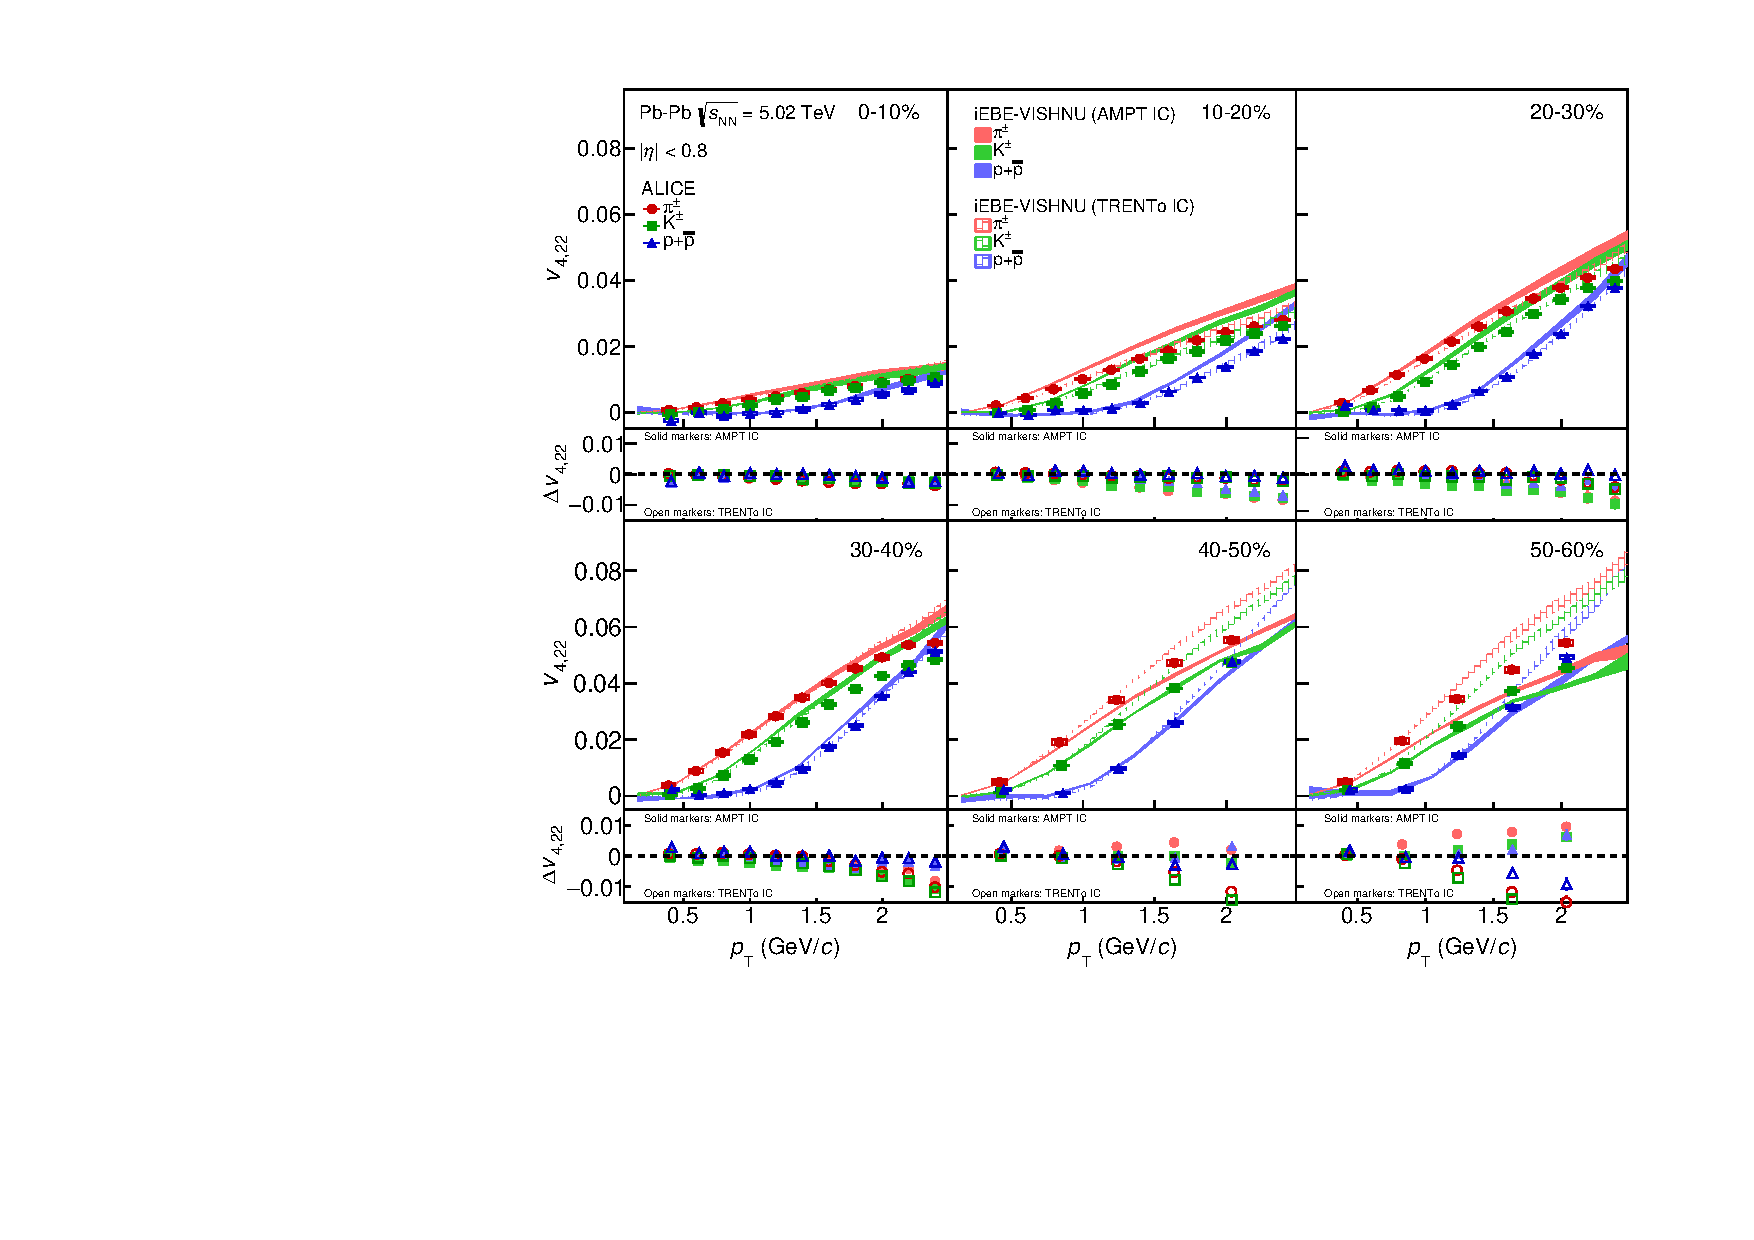
\includegraphics[scale=0.73]{figures/model/TrentoAndAMPT_v422_gap00_PID2.pdf}
\end{center}
\caption{The \pT-differential $v_{4,22}$ for different particle species in 10-20\% up to 50-60\% centrality intervals of Pb--Pb collisions at \sNN compared with iEBE-VISHNU hybrid models with two different sets of initial parameters: AMPT initial conditions ($\eta/s$= 0.08 and $\zeta/s$ = 0) shown in solid bands and TRENTo initial conditions ($\eta/s({\rm T})$ and $\zeta/s({\rm T})$) in hatched bands. The bottom panels show the difference between the measurements and each model.}
\label{v422_model}
\end{figure}


\begin{figure}[h]
\begin{center}
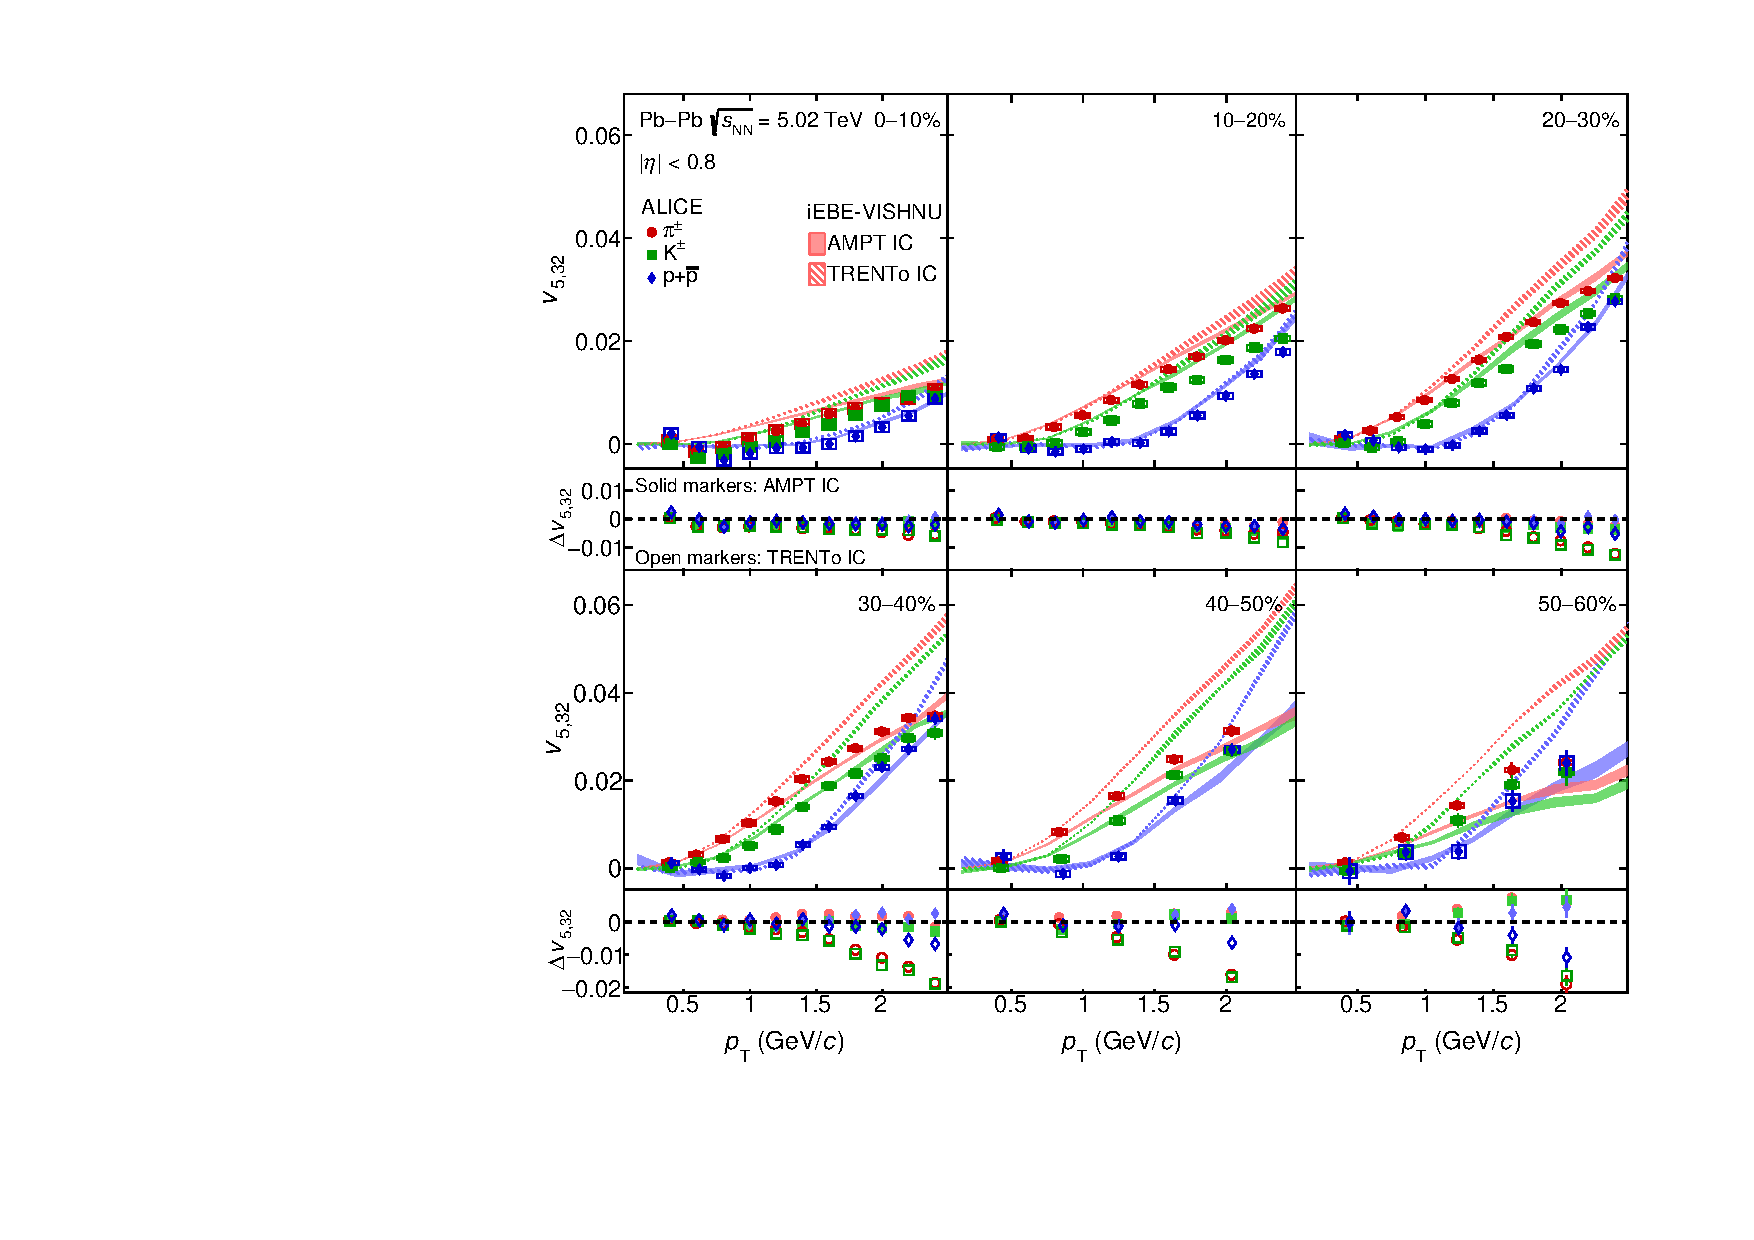
\includegraphics[scale=0.73]{figures/model/TrentoAndAMPT_v523_gap00_PID2.pdf}
\end{center}
\caption{The \pT-differential $v_{5,32}$ for different particle species in 10-20\% up to 50-60\% centrality intervals of Pb--Pb collisions at \sNN compared with iEBE-VISHNU hybrid models with two different sets of initial parameters: AMPT initial conditions ($\eta/s$= 0.08 and $\zeta/s$ = 0) shown in solid bands and TRENTo initial conditions ($\eta/s({\rm T})$ and $\zeta/s({\rm T})$) in hatched bands. The bottom panels show the difference between the measurements and each model.}
\label{v523_model}
\end{figure}

\begin{figure}[h]
\begin{center}
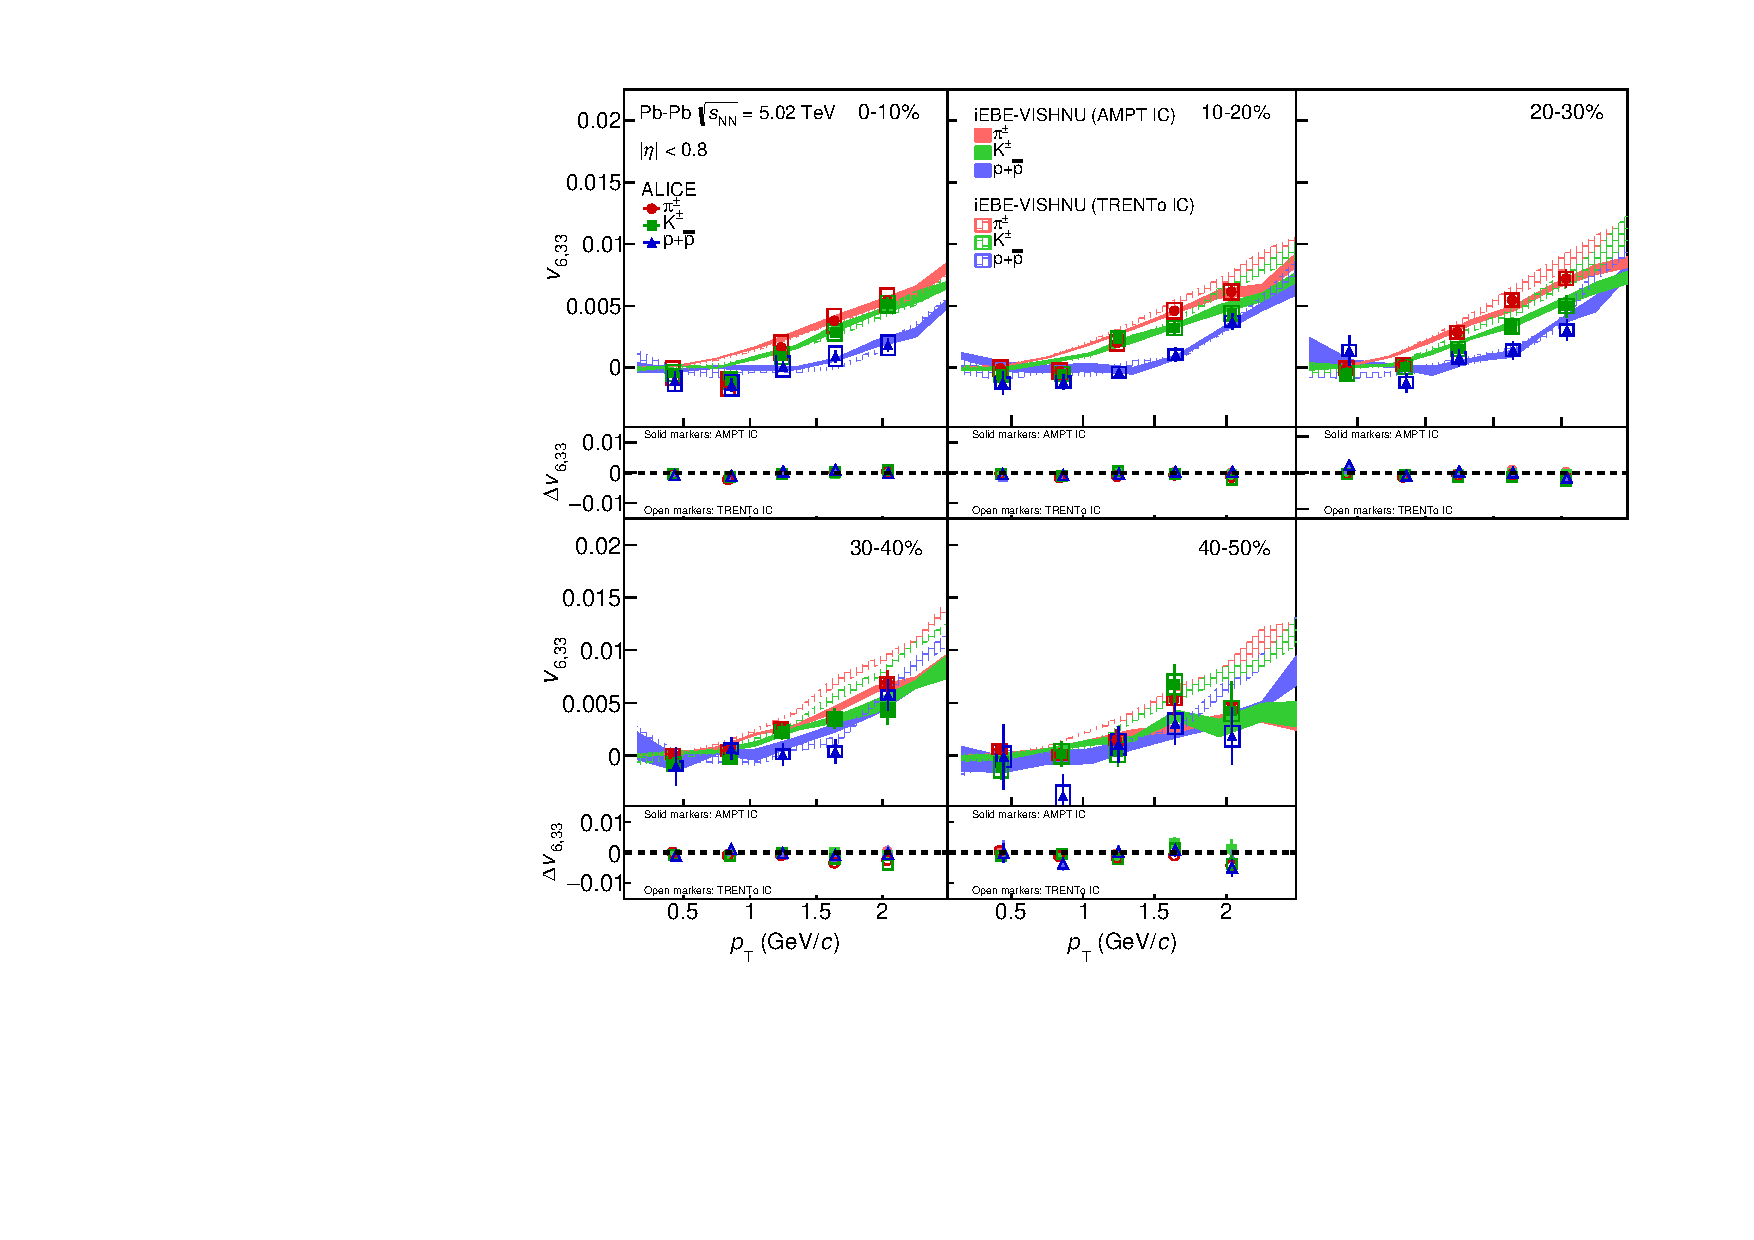
\includegraphics[scale=0.73]{figures/model/TrentoAndAMPT_v633_gap00_PID2.pdf}
\end{center}
\caption{The \pT-differential $v_{6,33}$ for different particle species in 10-20\% up to 40-50\% centrality intervals of Pb--Pb collisions at \sNN compared with iEBE-VISHNU hybrid models with two different sets of initial parameters: AMPT initial conditions ($\eta/s$= 0.08 and $\zeta/s$ = 0) shown in solid bands and TRENTo initial conditions ($\eta/s({\rm T})$ and $\zeta/s({\rm T})$) in hatched bands. The bottom panels show the difference between the measurements and each model.}
\label{v633_model}
\end{figure}


\begin{figure}[h]
\begin{center}
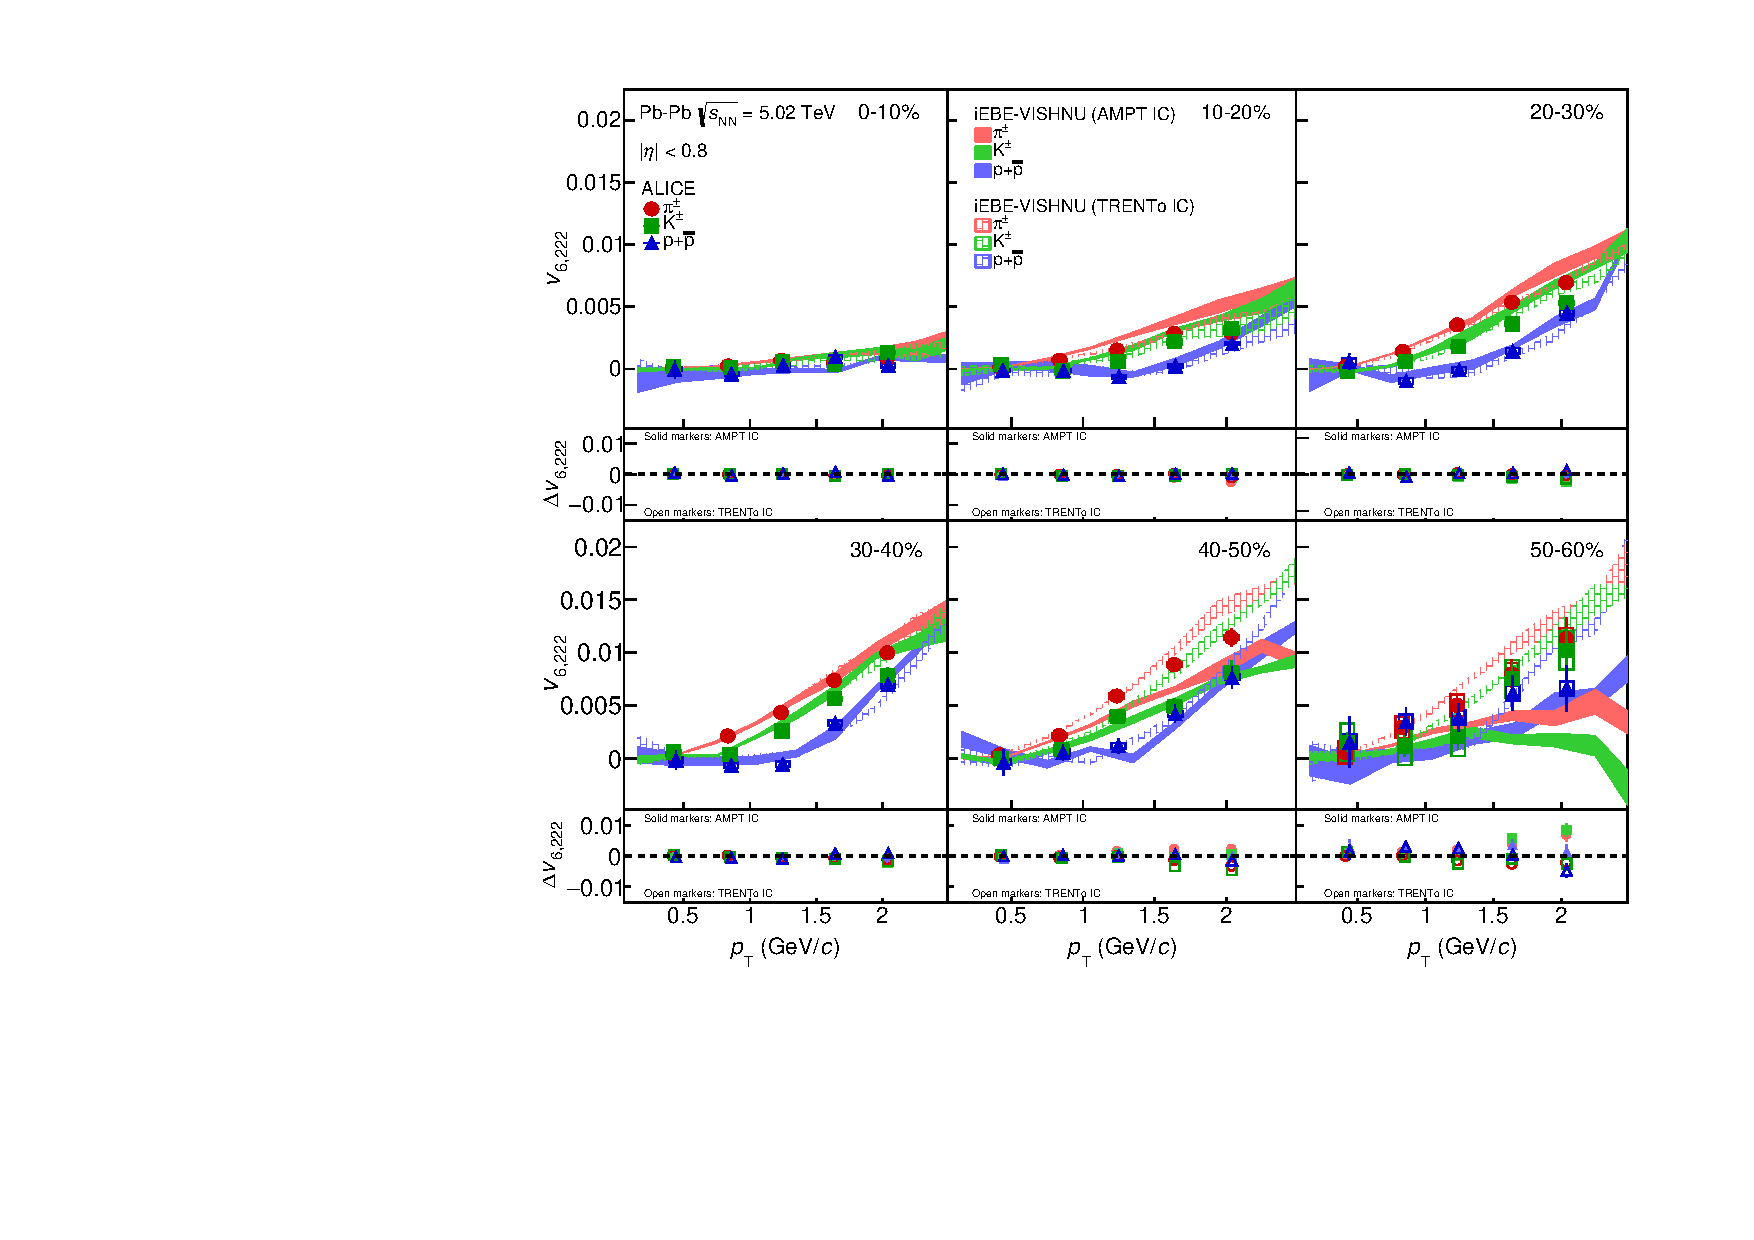
\includegraphics[scale=0.73]{figures/model/TrentoAndAMPT_v6222_gap00_PID2.pdf}
\end{center}
\caption{The \pT-differential $v_{6,222}$ for different particle species in 10-20\% up to 50-60\% centrality intervals of Pb--Pb collisions at \sNN compared with iEBE-VISHNU hybrid models with two different sets of initial parameters: AMPT initial conditions ($\eta/s$= 0.08 and $\zeta/s$ = 0) shown in solid bands and TRENTo initial conditions ($\eta/s({\rm T})$ and $\zeta/s({\rm T})$) in hatched bands. The bottom panels show the difference between the measurements and each model.}
\label{v6222_model}
\end{figure}


These two models have been utilised before to reproduce the \pT-differential $v_n$ measurements for identified particles \cite{Acharya:2018zuq}. In order to compare the performance of these two models in $v_n$ and $v_{n,mk}$ measurements, the relative ratios between each model and the measurements have been obtained. Tables \ref{ModelDataComparisonNLflow} and \ref{ModelDataComparisonflow} summarize these relative ratios for $v_{n,mk}$ and $v_{n}$, respectively. The ranges in these tables present the minimum and maximum value of a constant fit to the relative ratios obtained from most-central to mid-peripheral collisions. These values should be taken with caution as the non-linear flow modes have smaller magnitude and any discrepancy between the models and the data becomes magnified in the ratios. Comparison between Tab. \ref{ModelDataComparisonNLflow} and \ref{ModelDataComparisonflow} shows that the AMPT calculations reproduces $v_{4,22}$ with $\sim$20\% higher discrepancy on average compared to $v_{4}$, while, TRENTo calculations performs better in $v_{4,22}$ compared to $v_{4}$ with $\sim$7\%.  

All in all, this study shows larger discrepancy between the model calculations and $v_{n,mk}$ measurements wrt. that of $v_{n}$, indicating a larger sensitivity to the initial conditions and transport properties in non-linear flow modes. As a result, it is useful to tune the input parameters of hydrodynamic models using the non-linear flow measurements and constrain the values of transport properties and the initial conditions of the system.

%All in all, comparing this effort to the data-model comparison for anisotropic flow coefficients \cite{Acharya:2018zuq} shows that non-linear modes are more sensitive to the initial conditions and transport properties. However, similar to model-data comparisons for anisotropic flow, neither of the models can reproduce the data for all centrality intervals and particle species. As a result, in order to constrain the values of transport properties and the initial conditions of the system, it is necessary to tune the input parameters of hydrodynamic models using these measurements.



\begin{table}[!h]
\resizebox{\textwidth}{!}{\begin{tabular}{ |p{4.5cm} |l|c|c|c|c|c|c|c|c|c|c|c|c|}
\hline
\multicolumn{1}{| c |}{} & \multicolumn{3}{| c |}{ $v_{4,22}$ } & \multicolumn{3}{| c |}{ $v_{5,32}$} & \multicolumn{3}{| c |}{ $v_{6,33}$} & \multicolumn{3}{| c |}{ $v_{6,222}$} \\
\hline
Error source  & \pion &  \kaon & \proton &  \pion & \kaon & \proton &  \pion &  \kaon & \proton &  \pion &  \kaon & \proton \\ \hline  \hline
AMPT claculations &  5-30\% & 2-30\%  & 3-30\% & 3-28\%  & 5-29\% &  1-65\% & 0-46\% & 0-46\% & 0-97\% & 6-52\% & 0-80\%  & 0-118\% \\
TRENTo calculations & 0-30\% & 4-33\% & 0-21\% &  24-49\% & 33-97\% & 12-58\% & 0-43\% & 0-46\% & 0-95\% & 0-20\% & 0-34\% & 0-78\%\\
 \hline
\end{tabular}}
\caption{List of minimum and maximum value of the fit to relative ratios between the data and each model for  $v_{n,mk}$ of \pion, \kaon~and \proton. The minimum and maximum are obtained from 0-10\% up to 50-60\% (40-50\% for $v_{6,33}$) centrality intervals .}\label{ModelDataComparisonNLflow}
\end{table}



\begin{table}[!h]
\centering
\resizebox{0.78\textwidth}{!}{\begin{tabular}{ |p{4.5cm} |l|c|c|c|c|c|c|c|c|c|}
\hline
\multicolumn{1}{| c |}{} & \multicolumn{3}{| c |}{ $v_{2}$ } & \multicolumn{3}{| c |}{ $v_{3}$} & \multicolumn{3}{| c |}{ $v_{4}$}  \\
\hline
Error source  & \pion &  \kaon & \proton &  \pion & \kaon & \proton &  \pion &  \kaon & \proton \\ \hline  \hline
AMPT calculations & 3-13\% & 0-16\% & 0-20\% & 0-8\% & 5-12\% & 0-4\%& 0-7\% & 5-12\% & 0-4\%  \\
TRENTo calculations & 6-17\% & 0-19\% & 3-19\% & 2-15\% & 7-22\% & 0-11\% & 7-25\% & 16-28\% & 0-21\% \\
 \hline
\end{tabular}}
\caption{List of minimum and maximum value of the fit to relative ratios between the data and each model for  $v_{n} (n=2,3,4)$  of \pion, \kaon~and \proton. The minimum and maximum are obtained from 0-5\% up to 40-50\% centrality intervals .}\label{ModelDataComparisonflow}
\end{table}

\subsection{Comparison with $v_{n}$ of identified particles}
\label{SubSec:comparewithvn}

The features seen in the measurement of non-linear flow modes can be further studied by comparing to that of anisotropic flow coefficients. Such comparisons have been performed for $v_{4,22}$(\pT) (this study) and $v_{4}$(\pT) measurements \cite{Acharya:2018zuq} by taking the relative difference of pions wrt protons at a given \pT~in both modes. This comparison shows that the observed mass ordering in low \pT~region ($0$ <~\pT~< $2.5$ \GeV) is of the same magnitude in $v_{4,22}$ and $v_{4}$. In the intermediate \pT~region (\pT~> 2.5 \GeV), the same comparison shows similar particle type grouping in  $v_{4,22}$ and $v_{4}$ measurements. 

\newpage